% Options for packages loaded elsewhere
\PassOptionsToPackage{unicode}{hyperref}
\PassOptionsToPackage{hyphens}{url}
%
\documentclass[
]{article}
\usepackage{amsmath,amssymb}
\usepackage{iftex}
\ifPDFTeX
  \usepackage[T1]{fontenc}
  \usepackage[utf8]{inputenc}
  \usepackage{textcomp} % provide euro and other symbols
\else % if luatex or xetex
  \usepackage{unicode-math} % this also loads fontspec
  \defaultfontfeatures{Scale=MatchLowercase}
  \defaultfontfeatures[\rmfamily]{Ligatures=TeX,Scale=1}
\fi
\usepackage{lmodern}
\ifPDFTeX\else
  % xetex/luatex font selection
\fi
% Use upquote if available, for straight quotes in verbatim environments
\IfFileExists{upquote.sty}{\usepackage{upquote}}{}
\IfFileExists{microtype.sty}{% use microtype if available
  \usepackage[]{microtype}
  \UseMicrotypeSet[protrusion]{basicmath} % disable protrusion for tt fonts
}{}
\makeatletter
\@ifundefined{KOMAClassName}{% if non-KOMA class
  \IfFileExists{parskip.sty}{%
    \usepackage{parskip}
  }{% else
    \setlength{\parindent}{0pt}
    \setlength{\parskip}{6pt plus 2pt minus 1pt}}
}{% if KOMA class
  \KOMAoptions{parskip=half}}
\makeatother
\usepackage{xcolor}
\usepackage[margin=1in]{geometry}
\usepackage{longtable,booktabs,array}
\usepackage{calc} % for calculating minipage widths
% Correct order of tables after \paragraph or \subparagraph
\usepackage{etoolbox}
\makeatletter
\patchcmd\longtable{\par}{\if@noskipsec\mbox{}\fi\par}{}{}
\makeatother
% Allow footnotes in longtable head/foot
\IfFileExists{footnotehyper.sty}{\usepackage{footnotehyper}}{\usepackage{footnote}}
\makesavenoteenv{longtable}
\usepackage{graphicx}
\makeatletter
\def\maxwidth{\ifdim\Gin@nat@width>\linewidth\linewidth\else\Gin@nat@width\fi}
\def\maxheight{\ifdim\Gin@nat@height>\textheight\textheight\else\Gin@nat@height\fi}
\makeatother
% Scale images if necessary, so that they will not overflow the page
% margins by default, and it is still possible to overwrite the defaults
% using explicit options in \includegraphics[width, height, ...]{}
\setkeys{Gin}{width=\maxwidth,height=\maxheight,keepaspectratio}
% Set default figure placement to htbp
\makeatletter
\def\fps@figure{htbp}
\makeatother
\setlength{\emergencystretch}{3em} % prevent overfull lines
\providecommand{\tightlist}{%
  \setlength{\itemsep}{0pt}\setlength{\parskip}{0pt}}
\setcounter{secnumdepth}{-\maxdimen} % remove section numbering
\ifLuaTeX
  \usepackage{selnolig}  % disable illegal ligatures
\fi
\usepackage{bookmark}
\IfFileExists{xurl.sty}{\usepackage{xurl}}{} % add URL line breaks if available
\urlstyle{same}
\hypersetup{
  pdftitle={Actividad2 Unidad 2 InformeEjecutivo},
  pdfauthor={Juan José Restrepo Rosero},
  hidelinks,
  pdfcreator={LaTeX via pandoc}}

\title{Actividad2 Unidad 2 InformeEjecutivo}
\author{Juan José Restrepo Rosero}
\date{2025-03-03}

\begin{document}
\maketitle

{
\setcounter{tocdepth}{2}
\tableofcontents
}
\textbf{Caso C\&A}

Enunciado

Maria comenzó como agente de bienes raíces en Cali hace 10 años. Después
de laborar dos años para una empresa nacional, se traslado a Bogotá y
trabajó para otra agencia de bienes raíces. Sus amigos y familiares la
convencieron de que con su experiencia y conocimientos del negocio debía
abrir su propia agencia. Terminó por adquirir la licencia de
intermediario y al poco tiempo fundó su propia compañía, C\&A (Casas y
Apartamentos) en Cali. Santiago y Lina, dos vendedores de la empresa
anterior aceptaron trabajar en la nueva compaña. En la actualidad ocho
agentes de bienes raíces colaboran con ella en C\&A.

Actualmente las ventas de bienes raíces en Cali se han visto disminuidas
de manera significativa en lo corrido del año. Durante este periodo
muchas instituciones bancarias de ahorro y vivienda están prestando
grandes sumas de dinero para la industria y la construcción comercial y
residencial. Cuando el efecto producto de las tensiones políticas y
sociales disminuya, se espera que la actividad económica de este sector
se reactive.

Hace dos días, María recibió una carta solicitando asesoría para la
compra de dos viviendas por parte de una compañía internacional que
desea ubicar a dos de sus empleados con sus familias en la ciudad. Las
solicitudes incluyen las siguientes condiciones:

\begin{figure}
\centering
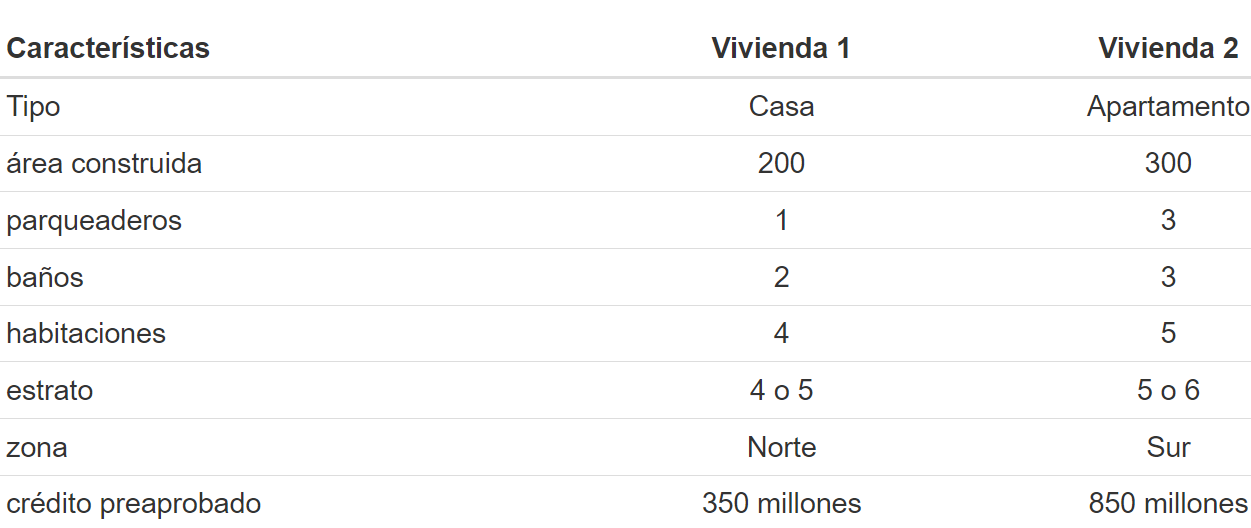
\includegraphics{C:/Users/Juan Jose Restrepo/Desktop/Master-Data-Science-main/Semestre 2/Modelos Estadisticos/A2_U2_InformeEjecutivo_JJRR/condiciones.png}
\caption{Condiciones}
\end{figure}

Pasos requeridos para la obtención de los resultados

Realice un filtro a la base de datos e incluya solo las ofertas de :
base1: casas, de la zona norte de la ciudad. Presente los primeros 3
registros de las bases y algunas tablas que comprueben la consulta.
(Adicional un mapa con los puntos de las bases. Discutir si todos los
puntos se ubican en la zona correspondiente o se presentan valores en
otras zonas, por que?).

Realice un análisis exploratorio de datos enfocado en la correlación
entre la variable respuesta (precio de la casa) en función del área
construida, estrato, numero de baños, numero de habitaciones y zona
donde se ubica la vivienda. Use gráficos interactivos con el paquete
plotly e interprete los resultados.

Estime un modelo de regresión lineal múltiple con las variables del
punto anterior (precio = f(área construida, estrato, número de cuartos,
número de parqueaderos, número de baños ) ) e interprete los
coeficientes si son estadísticamente significativos. Las
interpretaciones deber están contextualizadas y discutir si los
resultados son lógicos. Adicionalmente interprete el coeficiente R2 y
discuta el ajuste del modelo e implicaciones (que podrían hacer para
mejorarlo).

Realice la validación de supuestos del modelo e interprete los
resultados (no es necesario corregir en caso de presentar problemas,
solo realizar sugerencias de que se podría hacer).

Con el modelo identificado debe predecir el precio de la vivienda con
las características de la primera solicitud.

Con las predicciones del modelo sugiera potenciales ofertas que responda
a la solicitud de la vivienda 1. Tenga encuentra que la empresa tiene
crédito pre-aprobado de máximo 350 millones de pesos. Realice un
análisis y presente en un mapa al menos 5 ofertas potenciales que debe
discutir.

Realice los pasos del 1 al 6. Para la segunda solicitud que tiene un
crédito pre-aprobado por valor de \$850 millones.

\subsection{Exploración inicial de
datos}\label{exploraciuxf3n-inicial-de-datos}

Basándonos en la información proporcionada por el resumen y la
estructura del conjunto de datos, podemos hacer varias observaciones
significativas. El conjunto de datos consta de 8322 observaciones con 13
variables. Algunas de estas variables tienen valores faltantes, como
piso, estrato, preciom, areaconst, parqueaderos, banios, habitaciones,
longitud y latitud, lo que sugiere la necesidad de manejar estos valores
faltantes antes de realizar análisis posteriores. Las variables zona,
piso, tipo y barrio son de naturaleza categórica, mientras que las
variables id, estrato, preciom, areaconst, parqueaderos, banios,
habitaciones, longitud y latitud son numéricas. Además, la presencia de
problemas detectados en los datos sugiere la posibilidad de
inconsistencias o errores que deben abordarse durante el análisis. En
resumen, este conjunto de datos proporciona una variedad de información
sobre propiedades inmobiliarias, incluidos detalles sobre su ubicación,
características y precios, pero requerirá un procesamiento cuidadoso
para garantizar su validez y utilidad en el análisis posterior.

\begin{verbatim}
##        id           zona               piso              estrato     
##  Min.   :   1   Length:8322        Length:8322        Min.   :3.000  
##  1st Qu.:2080   Class :character   Class :character   1st Qu.:4.000  
##  Median :4160   Mode  :character   Mode  :character   Median :5.000  
##  Mean   :4160                                         Mean   :4.634  
##  3rd Qu.:6240                                         3rd Qu.:5.000  
##  Max.   :8319                                         Max.   :6.000  
##  NA's   :3                                            NA's   :3      
##     preciom         areaconst       parqueaderos        banios      
##  Min.   :  58.0   Min.   :  30.0   Min.   : 1.000   Min.   : 0.000  
##  1st Qu.: 220.0   1st Qu.:  80.0   1st Qu.: 1.000   1st Qu.: 2.000  
##  Median : 330.0   Median : 123.0   Median : 2.000   Median : 3.000  
##  Mean   : 433.9   Mean   : 174.9   Mean   : 1.835   Mean   : 3.111  
##  3rd Qu.: 540.0   3rd Qu.: 229.0   3rd Qu.: 2.000   3rd Qu.: 4.000  
##  Max.   :1999.0   Max.   :1745.0   Max.   :10.000   Max.   :10.000  
##  NA's   :2        NA's   :3        NA's   :1605     NA's   :3       
##   habitaciones        tipo              barrio             longitud     
##  Min.   : 0.000   Length:8322        Length:8322        Min.   :-76.59  
##  1st Qu.: 3.000   Class :character   Class :character   1st Qu.:-76.54  
##  Median : 3.000   Mode  :character   Mode  :character   Median :-76.53  
##  Mean   : 3.605                                         Mean   :-76.53  
##  3rd Qu.: 4.000                                         3rd Qu.:-76.52  
##  Max.   :10.000                                         Max.   :-76.46  
##  NA's   :3                                              NA's   :3       
##     latitud     
##  Min.   :3.333  
##  1st Qu.:3.381  
##  Median :3.416  
##  Mean   :3.418  
##  3rd Qu.:3.452  
##  Max.   :3.498  
##  NA's   :3
\end{verbatim}

\begin{verbatim}
## spc_tbl_ [8,322 x 13] (S3: spec_tbl_df/tbl_df/tbl/data.frame)
##  $ id          : num [1:8322] 1147 1169 1350 5992 1212 ...
##  $ zona        : chr [1:8322] "Zona Oriente" "Zona Oriente" "Zona Oriente" "Zona Sur" ...
##  $ piso        : chr [1:8322] NA NA NA "02" ...
##  $ estrato     : num [1:8322] 3 3 3 4 5 5 4 5 5 5 ...
##  $ preciom     : num [1:8322] 250 320 350 400 260 240 220 310 320 780 ...
##  $ areaconst   : num [1:8322] 70 120 220 280 90 87 52 137 150 380 ...
##  $ parqueaderos: num [1:8322] 1 1 2 3 1 1 2 2 2 2 ...
##  $ banios      : num [1:8322] 3 2 2 5 2 3 2 3 4 3 ...
##  $ habitaciones: num [1:8322] 6 3 4 3 3 3 3 4 6 3 ...
##  $ tipo        : chr [1:8322] "Casa" "Casa" "Casa" "Casa" ...
##  $ barrio      : chr [1:8322] "20 de julio" "20 de julio" "20 de julio" "3 de julio" ...
##  $ longitud    : num [1:8322] -76.5 -76.5 -76.5 -76.5 -76.5 ...
##  $ latitud     : num [1:8322] 3.43 3.43 3.44 3.44 3.46 ...
##  - attr(*, "spec")=
##   .. cols(
##   ..   id = col_double(),
##   ..   zona = col_character(),
##   ..   piso = col_character(),
##   ..   estrato = col_double(),
##   ..   preciom = col_double(),
##   ..   areaconst = col_double(),
##   ..   parqueaderos = col_double(),
##   ..   banios = col_double(),
##   ..   habitaciones = col_double(),
##   ..   tipo = col_character(),
##   ..   barrio = col_character(),
##   ..   longitud = col_double(),
##   ..   latitud = col_double()
##   .. )
##  - attr(*, "problems")=<externalptr>
\end{verbatim}

\subsection{1. Realice un filtro a la base de
datos}\label{realice-un-filtro-a-la-base-de-datos}

Base 1 Casas Zona Norte

De acuerdo a la solicitud del informe se presenta a continuación un sub
conjunto de datos que permite visualizar el contenido correspondiente al
tipo de inmueble casa para la zona norte, en este sentido se destaca lo
siguiente:

Las estadísticas descriptivas de las ofertas de casas en la zona norte
revelan una amplia gama de características y variabilidad en los datos.
Con un total de 722 registros, este conjunto de datos parece haber sido
filtrado correctamente para incluir solo las ofertas de casas en la zona
norte. Se observa la presencia de valores faltantes en algunos
atributos, lo cual es consistente con la estructura original del
dataset.

En cuanto a los precios de las casas, se observa una gran variación, con
precios que oscilan entre 58 y 1999 unidades monetarias. Tanto la
mediana como la media sugieren que la mayoría de las casas tienen
precios alrededor de 390 y 445.9 unidades monetarias, respectivamente.

El análisis del área construida revela una diversidad similar, con
valores que van desde 30 hasta 1745 metros cuadrados. La mediana y la
media indican que la mayoría de las casas tienen un área construida de
alrededor de 240 y 264.9 metros cuadrados, respectivamente.

Además de los precios y el área construida, otros atributos como el
número de parqueaderos, baños y habitaciones también varían
significativamente, con valores máximos de 10 en cada caso. Estos
atributos son cruciales para entender las características y comodidades
de las casas en la zona norte.

\begin{verbatim}
## Primeros 3 registros de la base de datos filtrada:
\end{verbatim}

\begin{longtable}[]{@{}
  >{\raggedleft\arraybackslash}p{(\columnwidth - 24\tabcolsep) * \real{0.0455}}
  >{\raggedright\arraybackslash}p{(\columnwidth - 24\tabcolsep) * \real{0.1000}}
  >{\raggedright\arraybackslash}p{(\columnwidth - 24\tabcolsep) * \real{0.0455}}
  >{\raggedleft\arraybackslash}p{(\columnwidth - 24\tabcolsep) * \real{0.0727}}
  >{\raggedleft\arraybackslash}p{(\columnwidth - 24\tabcolsep) * \real{0.0727}}
  >{\raggedleft\arraybackslash}p{(\columnwidth - 24\tabcolsep) * \real{0.0909}}
  >{\raggedleft\arraybackslash}p{(\columnwidth - 24\tabcolsep) * \real{0.1182}}
  >{\raggedleft\arraybackslash}p{(\columnwidth - 24\tabcolsep) * \real{0.0636}}
  >{\raggedleft\arraybackslash}p{(\columnwidth - 24\tabcolsep) * \real{0.1182}}
  >{\raggedright\arraybackslash}p{(\columnwidth - 24\tabcolsep) * \real{0.0455}}
  >{\raggedright\arraybackslash}p{(\columnwidth - 24\tabcolsep) * \real{0.0636}}
  >{\raggedleft\arraybackslash}p{(\columnwidth - 24\tabcolsep) * \real{0.0909}}
  >{\raggedleft\arraybackslash}p{(\columnwidth - 24\tabcolsep) * \real{0.0727}}@{}}
\toprule\noalign{}
\begin{minipage}[b]{\linewidth}\raggedleft
id
\end{minipage} & \begin{minipage}[b]{\linewidth}\raggedright
zona
\end{minipage} & \begin{minipage}[b]{\linewidth}\raggedright
piso
\end{minipage} & \begin{minipage}[b]{\linewidth}\raggedleft
estrato
\end{minipage} & \begin{minipage}[b]{\linewidth}\raggedleft
preciom
\end{minipage} & \begin{minipage}[b]{\linewidth}\raggedleft
areaconst
\end{minipage} & \begin{minipage}[b]{\linewidth}\raggedleft
parqueaderos
\end{minipage} & \begin{minipage}[b]{\linewidth}\raggedleft
banios
\end{minipage} & \begin{minipage}[b]{\linewidth}\raggedleft
habitaciones
\end{minipage} & \begin{minipage}[b]{\linewidth}\raggedright
tipo
\end{minipage} & \begin{minipage}[b]{\linewidth}\raggedright
barrio
\end{minipage} & \begin{minipage}[b]{\linewidth}\raggedleft
longitud
\end{minipage} & \begin{minipage}[b]{\linewidth}\raggedleft
latitud
\end{minipage} \\
\midrule\noalign{}
\endhead
\bottomrule\noalign{}
\endlastfoot
1209 & Zona Norte & 02 & 5 & 320 & 150 & 2 & 4 & 6 & Casa & acopi &
-76.51341 & 3.47968 \\
1592 & Zona Norte & 02 & 5 & 780 & 380 & 2 & 3 & 3 & Casa & acopi &
-76.51674 & 3.48721 \\
4057 & Zona Norte & 02 & 6 & 750 & 445 & NA & 7 & 6 & Casa & acopi &
-76.52950 & 3.38527 \\
\end{longtable}

\begin{verbatim}
## Estadísticas descriptivas de las ofertas de casas en la zona norte:
\end{verbatim}

\begin{longtable}[]{@{}
  >{\raggedright\arraybackslash}p{(\columnwidth - 26\tabcolsep) * \real{0.0147}}
  >{\raggedright\arraybackslash}p{(\columnwidth - 26\tabcolsep) * \real{0.0735}}
  >{\raggedright\arraybackslash}p{(\columnwidth - 26\tabcolsep) * \real{0.0833}}
  >{\raggedright\arraybackslash}p{(\columnwidth - 26\tabcolsep) * \real{0.0833}}
  >{\raggedright\arraybackslash}p{(\columnwidth - 26\tabcolsep) * \real{0.0686}}
  >{\raggedright\arraybackslash}p{(\columnwidth - 26\tabcolsep) * \real{0.0735}}
  >{\raggedright\arraybackslash}p{(\columnwidth - 26\tabcolsep) * \real{0.0735}}
  >{\raggedright\arraybackslash}p{(\columnwidth - 26\tabcolsep) * \real{0.0735}}
  >{\raggedright\arraybackslash}p{(\columnwidth - 26\tabcolsep) * \real{0.0735}}
  >{\raggedright\arraybackslash}p{(\columnwidth - 26\tabcolsep) * \real{0.0735}}
  >{\raggedright\arraybackslash}p{(\columnwidth - 26\tabcolsep) * \real{0.0833}}
  >{\raggedright\arraybackslash}p{(\columnwidth - 26\tabcolsep) * \real{0.0833}}
  >{\raggedright\arraybackslash}p{(\columnwidth - 26\tabcolsep) * \real{0.0735}}
  >{\raggedright\arraybackslash}p{(\columnwidth - 26\tabcolsep) * \real{0.0686}}@{}}
\toprule\noalign{}
\begin{minipage}[b]{\linewidth}\raggedright
\end{minipage} & \begin{minipage}[b]{\linewidth}\raggedright
id
\end{minipage} & \begin{minipage}[b]{\linewidth}\raggedright
zona
\end{minipage} & \begin{minipage}[b]{\linewidth}\raggedright
piso
\end{minipage} & \begin{minipage}[b]{\linewidth}\raggedright
estrato
\end{minipage} & \begin{minipage}[b]{\linewidth}\raggedright
preciom
\end{minipage} & \begin{minipage}[b]{\linewidth}\raggedright
areaconst
\end{minipage} & \begin{minipage}[b]{\linewidth}\raggedright
parqueaderos
\end{minipage} & \begin{minipage}[b]{\linewidth}\raggedright
banios
\end{minipage} & \begin{minipage}[b]{\linewidth}\raggedright
habitaciones
\end{minipage} & \begin{minipage}[b]{\linewidth}\raggedright
tipo
\end{minipage} & \begin{minipage}[b]{\linewidth}\raggedright
barrio
\end{minipage} & \begin{minipage}[b]{\linewidth}\raggedright
longitud
\end{minipage} & \begin{minipage}[b]{\linewidth}\raggedright
latitud
\end{minipage} \\
\midrule\noalign{}
\endhead
\bottomrule\noalign{}
\endlastfoot
& Min. : 58.0 & Length:722 & Length:722 & Min. :3.000 & Min. : 89.0 &
Min. : 30.0 & Min. : 1.000 & Min. : 0.000 & Min. : 0.000 & Length:722 &
Length:722 & Min. :-76.59 & Min. :3.333 \\
& 1st Qu.: 766.2 & Class :character & Class :character & 1st Qu.:3.000 &
1st Qu.: 261.2 & 1st Qu.: 140.0 & 1st Qu.: 1.000 & 1st Qu.: 2.000 & 1st
Qu.: 3.000 & Class :character & Class :character & 1st Qu.:-76.53 & 1st
Qu.:3.452 \\
& Median :2257.0 & Mode :character & Mode :character & Median :4.000 &
Median : 390.0 & Median : 240.0 & Median : 2.000 & Median : 3.000 &
Median : 4.000 & Mode :character & Mode :character & Median :-76.52 &
Median :3.468 \\
& Mean :2574.6 & NA & NA & Mean :4.202 & Mean : 445.9 & Mean : 264.9 &
Mean : 2.182 & Mean : 3.555 & Mean : 4.507 & NA & NA & Mean :-76.52 &
Mean :3.460 \\
& 3rd Qu.:4225.0 & NA & NA & 3rd Qu.:5.000 & 3rd Qu.: 550.0 & 3rd Qu.:
336.8 & 3rd Qu.: 3.000 & 3rd Qu.: 4.000 & 3rd Qu.: 5.000 & NA & NA & 3rd
Qu.:-76.50 & 3rd Qu.:3.482 \\
& Max. :8319.0 & NA & NA & Max. :6.000 & Max. :1940.0 & Max. :1440.0 &
Max. :10.000 & Max. :10.000 & Max. :10.000 & NA & NA & Max. :-76.47 &
Max. :3.496 \\
& NA & NA & NA & NA & NA & NA & NA's :287 & NA & NA & NA & NA & NA &
NA \\
\end{longtable}

El gráfico de dispersión indica una fuerte correlación positiva entre el
precio y el área construida de las casas en la Zona Norte. El
coeficiente de correlación de 0,73 evidencia esta relación directa,
donde a mayor área construida, mayor es el precio de la vivienda. La
línea de tendencia sugiere un incremento promedio de 1,35 millones de
pesos por metro cuadrado adicional. No obstante, la dispersión de los
puntos alrededor de la línea de tendencia revela variaciones en el
precio influenciadas por otros factores como la ubicación, calidad de
construcción, características de la casa y el mercado inmobiliario.
Considerar todos estos aspectos es crucial al momento de buscar una
vivienda en la Zona Norte.
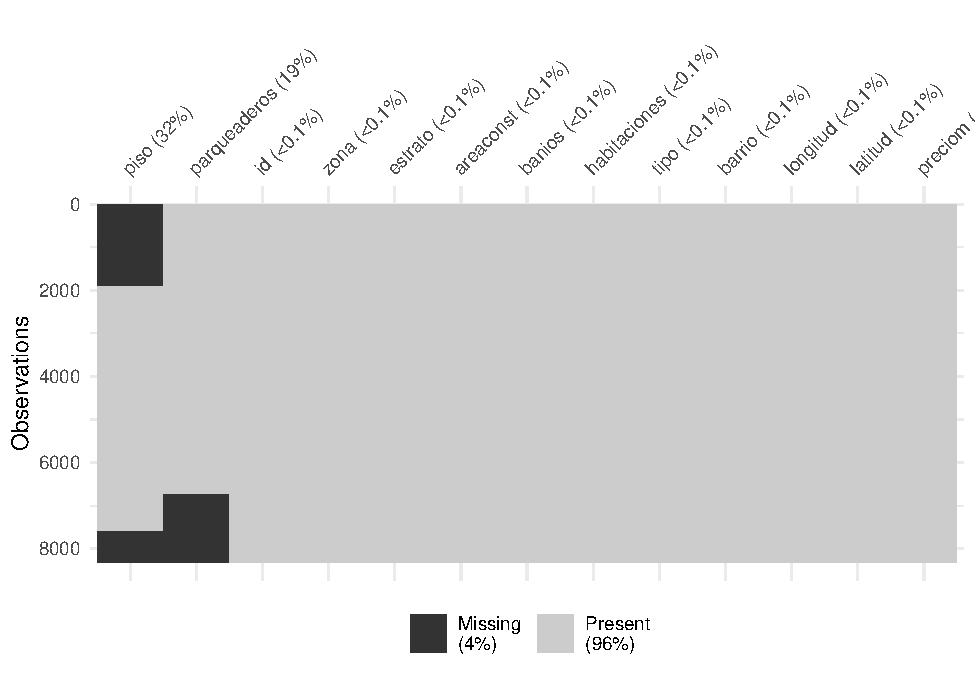
\includegraphics{A2_U2_InformeEjecutivo_files/figure-latex/unnamed-chunk-4-1.pdf}
\includegraphics{A2_U2_InformeEjecutivo_files/figure-latex/unnamed-chunk-4-2.pdf}

\begin{verbatim}
## Tabla de frecuencia de tipos de vivienda en la zona norte:
\end{verbatim}

\begin{longtable}[]{@{}lr@{}}
\toprule\noalign{}
Var1 & Freq \\
\midrule\noalign{}
\endhead
\bottomrule\noalign{}
\endlastfoot
Casa & 722 \\
\end{longtable}

\begin{verbatim}
## Tabla de frecuencia de estratos en la zona norte:
\end{verbatim}

\begin{longtable}[]{@{}lr@{}}
\toprule\noalign{}
Var1 & Freq \\
\midrule\noalign{}
\endhead
\bottomrule\noalign{}
\endlastfoot
3 & 235 \\
4 & 161 \\
5 & 271 \\
6 & 55 \\
\end{longtable}

\begin{verbatim}
## Tabla de frecuencia de barrios en la zona norte (ordenada por frecuencia descendente):
\end{verbatim}

\begin{longtable}[]{@{}lr@{}}
\toprule\noalign{}
Var1 & Freq \\
\midrule\noalign{}
\endhead
\bottomrule\noalign{}
\endlastfoot
acopi & 70 \\
brisas de los & 22 \\
alamos & 3 \\
barranquilla & 3 \\
base aérea & 2 \\
alameda del río & 1 \\
atanasio girardot & 1 \\
barrio tranquilo y & 1 \\
berlin & 1 \\
brisas del guabito & 1 \\
\end{longtable}

Base 2 Casas Zona Sur

Las estadísticas descriptivas de las ofertas de casas en la zona sur
muestran una diversidad significativa en los datos. Con un total de 1939
registros, este conjunto de datos parece haber sido filtrado
adecuadamente para incluir solo las ofertas de casas en la zona sur. Se
observa la presencia de valores faltantes en algunos atributos, lo cual
es consistente con la estructura original del dataset.

En relación a los precios de las casas, se evidencia una amplia
variación, con valores que oscilan entre 77 y 1900 unidades monetarias.
Tanto la mediana como la media sugieren que la mayoría de las casas
tienen precios alrededor de 480 y 612.3 unidades monetarias,
respectivamente.

El análisis del área construida también revela una diversidad similar,
con valores que van desde 48 hasta 1600 metros cuadrados. La mediana y
la media indican que la mayoría de las casas tienen un área construida
de alrededor de 247 y 282.3 metros cuadrados, respectivamente.

Además de los precios y el área construida, otros atributos como el
número de parqueaderos, baños y habitaciones también varían
significativamente, con valores máximos de 10 en cada caso. Estos
atributos son cruciales para comprender las características y
comodidades de las casas en la zona sur.

\begin{verbatim}
## Primeros 3 registros de la base de datos filtrada:
\end{verbatim}

\begin{longtable}[]{@{}
  >{\raggedleft\arraybackslash}p{(\columnwidth - 24\tabcolsep) * \real{0.0450}}
  >{\raggedright\arraybackslash}p{(\columnwidth - 24\tabcolsep) * \real{0.0811}}
  >{\raggedright\arraybackslash}p{(\columnwidth - 24\tabcolsep) * \real{0.0450}}
  >{\raggedleft\arraybackslash}p{(\columnwidth - 24\tabcolsep) * \real{0.0721}}
  >{\raggedleft\arraybackslash}p{(\columnwidth - 24\tabcolsep) * \real{0.0721}}
  >{\raggedleft\arraybackslash}p{(\columnwidth - 24\tabcolsep) * \real{0.0901}}
  >{\raggedleft\arraybackslash}p{(\columnwidth - 24\tabcolsep) * \real{0.1171}}
  >{\raggedleft\arraybackslash}p{(\columnwidth - 24\tabcolsep) * \real{0.0631}}
  >{\raggedleft\arraybackslash}p{(\columnwidth - 24\tabcolsep) * \real{0.1171}}
  >{\raggedright\arraybackslash}p{(\columnwidth - 24\tabcolsep) * \real{0.0450}}
  >{\raggedright\arraybackslash}p{(\columnwidth - 24\tabcolsep) * \real{0.0991}}
  >{\raggedleft\arraybackslash}p{(\columnwidth - 24\tabcolsep) * \real{0.0811}}
  >{\raggedleft\arraybackslash}p{(\columnwidth - 24\tabcolsep) * \real{0.0721}}@{}}
\toprule\noalign{}
\begin{minipage}[b]{\linewidth}\raggedleft
id
\end{minipage} & \begin{minipage}[b]{\linewidth}\raggedright
zona
\end{minipage} & \begin{minipage}[b]{\linewidth}\raggedright
piso
\end{minipage} & \begin{minipage}[b]{\linewidth}\raggedleft
estrato
\end{minipage} & \begin{minipage}[b]{\linewidth}\raggedleft
preciom
\end{minipage} & \begin{minipage}[b]{\linewidth}\raggedleft
areaconst
\end{minipage} & \begin{minipage}[b]{\linewidth}\raggedleft
parqueaderos
\end{minipage} & \begin{minipage}[b]{\linewidth}\raggedleft
banios
\end{minipage} & \begin{minipage}[b]{\linewidth}\raggedleft
habitaciones
\end{minipage} & \begin{minipage}[b]{\linewidth}\raggedright
tipo
\end{minipage} & \begin{minipage}[b]{\linewidth}\raggedright
barrio
\end{minipage} & \begin{minipage}[b]{\linewidth}\raggedleft
longitud
\end{minipage} & \begin{minipage}[b]{\linewidth}\raggedleft
latitud
\end{minipage} \\
\midrule\noalign{}
\endhead
\bottomrule\noalign{}
\endlastfoot
5992 & Zona Sur & 02 & 4 & 400 & 280 & 3 & 5 & 3 & Casa & 3 de julio &
-76.540 & 3.435 \\
5157 & Zona Sur & 02 & 3 & 500 & 354 & 1 & 2 & 4 & Casa & alameda &
-76.535 & 3.437 \\
5501 & Zona Sur & 02 & 3 & 175 & 102 & NA & 2 & 4 & Casa & alameda &
-76.537 & 3.435 \\
\end{longtable}

\begin{verbatim}
## Estadísticas descriptivas de las ofertas de casas en la zona sur:
\end{verbatim}

\begin{longtable}[]{@{}
  >{\raggedright\arraybackslash}p{(\columnwidth - 26\tabcolsep) * \real{0.0149}}
  >{\raggedright\arraybackslash}p{(\columnwidth - 26\tabcolsep) * \real{0.0644}}
  >{\raggedright\arraybackslash}p{(\columnwidth - 26\tabcolsep) * \real{0.0842}}
  >{\raggedright\arraybackslash}p{(\columnwidth - 26\tabcolsep) * \real{0.0842}}
  >{\raggedright\arraybackslash}p{(\columnwidth - 26\tabcolsep) * \real{0.0693}}
  >{\raggedright\arraybackslash}p{(\columnwidth - 26\tabcolsep) * \real{0.0743}}
  >{\raggedright\arraybackslash}p{(\columnwidth - 26\tabcolsep) * \real{0.0743}}
  >{\raggedright\arraybackslash}p{(\columnwidth - 26\tabcolsep) * \real{0.0743}}
  >{\raggedright\arraybackslash}p{(\columnwidth - 26\tabcolsep) * \real{0.0743}}
  >{\raggedright\arraybackslash}p{(\columnwidth - 26\tabcolsep) * \real{0.0743}}
  >{\raggedright\arraybackslash}p{(\columnwidth - 26\tabcolsep) * \real{0.0842}}
  >{\raggedright\arraybackslash}p{(\columnwidth - 26\tabcolsep) * \real{0.0842}}
  >{\raggedright\arraybackslash}p{(\columnwidth - 26\tabcolsep) * \real{0.0743}}
  >{\raggedright\arraybackslash}p{(\columnwidth - 26\tabcolsep) * \real{0.0693}}@{}}
\toprule\noalign{}
\begin{minipage}[b]{\linewidth}\raggedright
\end{minipage} & \begin{minipage}[b]{\linewidth}\raggedright
id
\end{minipage} & \begin{minipage}[b]{\linewidth}\raggedright
zona
\end{minipage} & \begin{minipage}[b]{\linewidth}\raggedright
piso
\end{minipage} & \begin{minipage}[b]{\linewidth}\raggedright
estrato
\end{minipage} & \begin{minipage}[b]{\linewidth}\raggedright
preciom
\end{minipage} & \begin{minipage}[b]{\linewidth}\raggedright
areaconst
\end{minipage} & \begin{minipage}[b]{\linewidth}\raggedright
parqueaderos
\end{minipage} & \begin{minipage}[b]{\linewidth}\raggedright
banios
\end{minipage} & \begin{minipage}[b]{\linewidth}\raggedright
habitaciones
\end{minipage} & \begin{minipage}[b]{\linewidth}\raggedright
tipo
\end{minipage} & \begin{minipage}[b]{\linewidth}\raggedright
barrio
\end{minipage} & \begin{minipage}[b]{\linewidth}\raggedright
longitud
\end{minipage} & \begin{minipage}[b]{\linewidth}\raggedright
latitud
\end{minipage} \\
\midrule\noalign{}
\endhead
\bottomrule\noalign{}
\endlastfoot
& Min. : 1 & Length:1939 & Length:1939 & Min. :3.000 & Min. : 77.0 &
Min. : 48.0 & Min. : 1.000 & Min. : 0.000 & Min. : 0.000 & Length:1939 &
Length:1939 & Min. :-76.57 & Min. :3.333 \\
& 1st Qu.:3230 & Class :character & Class :character & 1st Qu.:4.000 &
1st Qu.: 350.0 & 1st Qu.: 163.5 & 1st Qu.: 1.000 & 1st Qu.: 3.000 & 1st
Qu.: 3.000 & Class :character & Class :character & 1st Qu.:-76.54 & 1st
Qu.:3.368 \\
& Median :4941 & Mode :character & Mode :character & Median :5.000 &
Median : 480.0 & Median : 247.0 & Median : 2.000 & Median : 4.000 &
Median : 4.000 & Mode :character & Mode :character & Median :-76.53 &
Median :3.389 \\
& Mean :4691 & NA & NA & Mean :4.842 & Mean : 612.3 & Mean : 282.3 &
Mean : 2.415 & Mean : 4.173 & Mean : 4.514 & NA & NA & Mean :-76.53 &
Mean :3.391 \\
& 3rd Qu.:6264 & NA & NA & 3rd Qu.:6.000 & 3rd Qu.: 780.0 & 3rd Qu.:
350.0 & 3rd Qu.: 3.000 & 3rd Qu.: 5.000 & 3rd Qu.: 5.000 & NA & NA & 3rd
Qu.:-76.53 & 3rd Qu.:3.413 \\
& Max. :8305 & NA & NA & Max. :6.000 & Max. :1900.0 & Max. :1600.0 &
Max. :10.000 & Max. :10.000 & Max. :10.000 & NA & NA & Max. :-76.46 &
Max. :3.485 \\
& NA & NA & NA & NA & NA & NA & NA's :215 & NA & NA & NA & NA & NA &
NA \\
\end{longtable}

El gráfico de dispersión para la Zona Sur presenta un coeficiente de
correlación de 0.67, lo que indica una fuerte correlación positiva entre
el precio y el área construida. Esto significa que existe una relación
directa entre ambas variables: a mayor área construida, mayor es el
precio de la vivienda.

La línea de tendencia en el gráfico indica que, en promedio, el precio
aumenta en 1.2 millones de pesos por cada metro cuadrado adicional de
área construida.

Sin embargo, la dispersión de los puntos alrededor de la línea de
tendencia muestra una variación considerable en los precios.

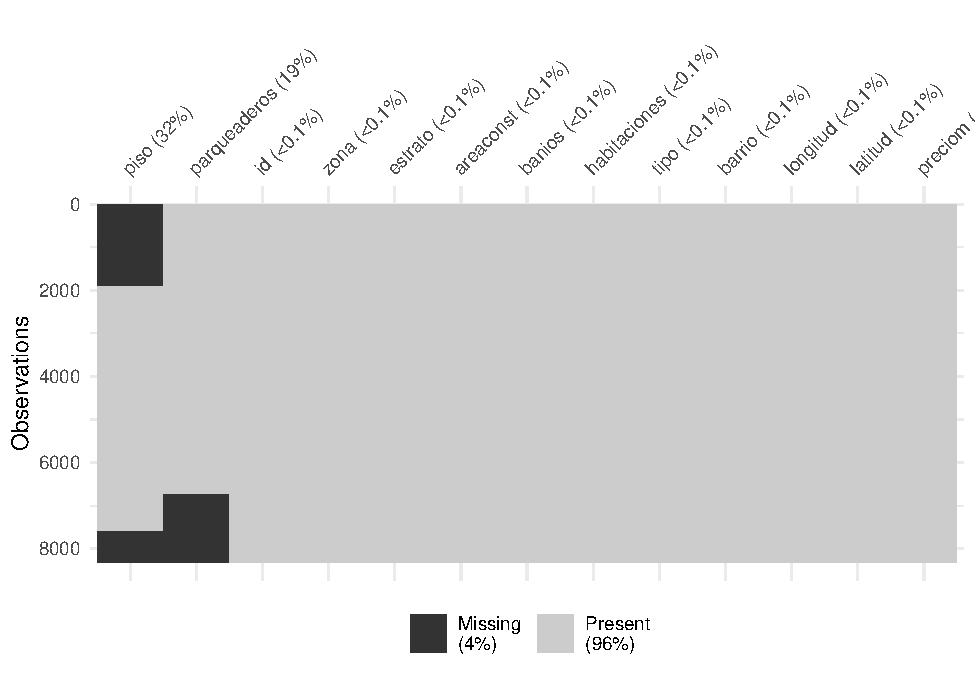
\includegraphics{A2_U2_InformeEjecutivo_files/figure-latex/unnamed-chunk-6-1.pdf}
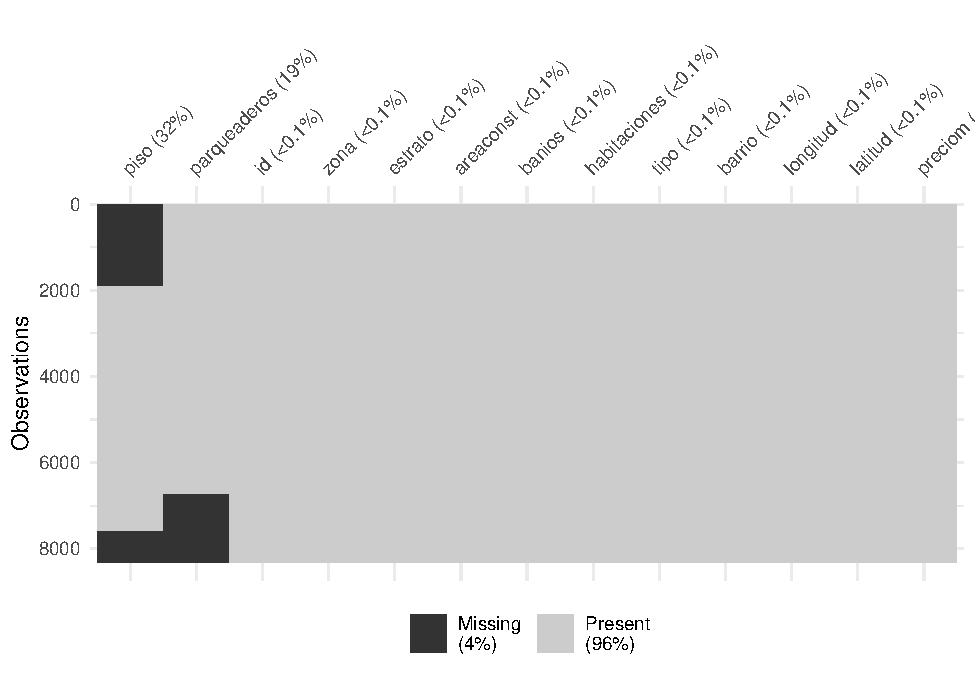
\includegraphics{A2_U2_InformeEjecutivo_files/figure-latex/unnamed-chunk-6-2.pdf}

\begin{verbatim}
## Tabla de frecuencia de tipos de vivienda en la zona sur:
\end{verbatim}

\begin{longtable}[]{@{}lr@{}}
\toprule\noalign{}
Var1 & Freq \\
\midrule\noalign{}
\endhead
\bottomrule\noalign{}
\endlastfoot
Casa & 1939 \\
\end{longtable}

\begin{verbatim}
## Tabla de frecuencia de estratos en la zona sur:
\end{verbatim}

\begin{longtable}[]{@{}lr@{}}
\toprule\noalign{}
Var1 & Freq \\
\midrule\noalign{}
\endhead
\bottomrule\noalign{}
\endlastfoot
3 & 181 \\
4 & 525 \\
5 & 652 \\
6 & 581 \\
\end{longtable}

\begin{verbatim}
## Tabla de frecuencia de barrios en la zona sur (ordenada por frecuencia descendente):
\end{verbatim}

\begin{longtable}[]{@{}lr@{}}
\toprule\noalign{}
Var1 & Freq \\
\midrule\noalign{}
\endhead
\bottomrule\noalign{}
\endlastfoot
alameda & 3 \\
altos de guadalupe & 2 \\
bella suiza alta & 2 \\
3 de julio & 1 \\
alborada & 1 \\
alférez real & 1 \\
alferez real & 1 \\
aranjuez & 1 \\
barrio eucarístico & 1 \\
belalcazar & 1 \\
\end{longtable}

Base 3 Casas Zona Oriente

Las estadísticas descriptivas de las ofertas de casas en la zona oriente
muestran una distribución similar en los datos. Con un total de 289
registros, se observa una variabilidad notable en los atributos
considerados. Al igual que en otras zonas, se encuentran valores
faltantes en algunos atributos, lo cual es coherente con la estructura
original del dataset.

En cuanto a los precios de las casas, se observa una variación
considerable, con valores que van desde 80 hasta 750 unidades
monetarias. Tanto la mediana como la media sugieren que la mayoría de
las casas tienen precios alrededor de 235 y 244.8 unidades monetarias,
respectivamente.

El análisis del área construida también muestra una diversidad
significativa, con valores que van desde 40 hasta 1745 metros cuadrados.
La mediana y la media indican que la mayoría de las casas tienen un área
construida de alrededor de 179 y 213.4 metros cuadrados,
respectivamente.

Además de los precios y el área construida, otros atributos como el
número de parqueaderos, baños y habitaciones también exhiben variaciones
notables, con valores máximos de 10 en cada caso.

\begin{verbatim}
## Primeros 3 registros de la base de datos filtrada:
\end{verbatim}

\begin{longtable}[]{@{}
  >{\raggedleft\arraybackslash}p{(\columnwidth - 24\tabcolsep) * \real{0.0427}}
  >{\raggedright\arraybackslash}p{(\columnwidth - 24\tabcolsep) * \real{0.1111}}
  >{\raggedright\arraybackslash}p{(\columnwidth - 24\tabcolsep) * \real{0.0427}}
  >{\raggedleft\arraybackslash}p{(\columnwidth - 24\tabcolsep) * \real{0.0684}}
  >{\raggedleft\arraybackslash}p{(\columnwidth - 24\tabcolsep) * \real{0.0684}}
  >{\raggedleft\arraybackslash}p{(\columnwidth - 24\tabcolsep) * \real{0.0855}}
  >{\raggedleft\arraybackslash}p{(\columnwidth - 24\tabcolsep) * \real{0.1111}}
  >{\raggedleft\arraybackslash}p{(\columnwidth - 24\tabcolsep) * \real{0.0598}}
  >{\raggedleft\arraybackslash}p{(\columnwidth - 24\tabcolsep) * \real{0.1111}}
  >{\raggedright\arraybackslash}p{(\columnwidth - 24\tabcolsep) * \real{0.0427}}
  >{\raggedright\arraybackslash}p{(\columnwidth - 24\tabcolsep) * \real{0.1026}}
  >{\raggedleft\arraybackslash}p{(\columnwidth - 24\tabcolsep) * \real{0.0855}}
  >{\raggedleft\arraybackslash}p{(\columnwidth - 24\tabcolsep) * \real{0.0684}}@{}}
\toprule\noalign{}
\begin{minipage}[b]{\linewidth}\raggedleft
id
\end{minipage} & \begin{minipage}[b]{\linewidth}\raggedright
zona
\end{minipage} & \begin{minipage}[b]{\linewidth}\raggedright
piso
\end{minipage} & \begin{minipage}[b]{\linewidth}\raggedleft
estrato
\end{minipage} & \begin{minipage}[b]{\linewidth}\raggedleft
preciom
\end{minipage} & \begin{minipage}[b]{\linewidth}\raggedleft
areaconst
\end{minipage} & \begin{minipage}[b]{\linewidth}\raggedleft
parqueaderos
\end{minipage} & \begin{minipage}[b]{\linewidth}\raggedleft
banios
\end{minipage} & \begin{minipage}[b]{\linewidth}\raggedleft
habitaciones
\end{minipage} & \begin{minipage}[b]{\linewidth}\raggedright
tipo
\end{minipage} & \begin{minipage}[b]{\linewidth}\raggedright
barrio
\end{minipage} & \begin{minipage}[b]{\linewidth}\raggedleft
longitud
\end{minipage} & \begin{minipage}[b]{\linewidth}\raggedleft
latitud
\end{minipage} \\
\midrule\noalign{}
\endhead
\bottomrule\noalign{}
\endlastfoot
1147 & Zona Oriente & NA & 3 & 250 & 70 & 1 & 3 & 6 & Casa & 20 de julio
& -76.51168 & 3.43382 \\
1169 & Zona Oriente & NA & 3 & 320 & 120 & 1 & 2 & 3 & Casa & 20 de
julio & -76.51237 & 3.43369 \\
1350 & Zona Oriente & NA & 3 & 350 & 220 & 2 & 2 & 4 & Casa & 20 de
julio & -76.51537 & 3.43566 \\
\end{longtable}

\begin{verbatim}
## Estadísticas descriptivas de las ofertas de casas en la zona Oriente:
\end{verbatim}

\begin{longtable}[]{@{}
  >{\raggedright\arraybackslash}p{(\columnwidth - 26\tabcolsep) * \real{0.0150}}
  >{\raggedright\arraybackslash}p{(\columnwidth - 26\tabcolsep) * \real{0.0650}}
  >{\raggedright\arraybackslash}p{(\columnwidth - 26\tabcolsep) * \real{0.0850}}
  >{\raggedright\arraybackslash}p{(\columnwidth - 26\tabcolsep) * \real{0.0850}}
  >{\raggedright\arraybackslash}p{(\columnwidth - 26\tabcolsep) * \real{0.0700}}
  >{\raggedright\arraybackslash}p{(\columnwidth - 26\tabcolsep) * \real{0.0700}}
  >{\raggedright\arraybackslash}p{(\columnwidth - 26\tabcolsep) * \real{0.0750}}
  >{\raggedright\arraybackslash}p{(\columnwidth - 26\tabcolsep) * \real{0.0700}}
  >{\raggedright\arraybackslash}p{(\columnwidth - 26\tabcolsep) * \real{0.0750}}
  >{\raggedright\arraybackslash}p{(\columnwidth - 26\tabcolsep) * \real{0.0750}}
  >{\raggedright\arraybackslash}p{(\columnwidth - 26\tabcolsep) * \real{0.0850}}
  >{\raggedright\arraybackslash}p{(\columnwidth - 26\tabcolsep) * \real{0.0850}}
  >{\raggedright\arraybackslash}p{(\columnwidth - 26\tabcolsep) * \real{0.0750}}
  >{\raggedright\arraybackslash}p{(\columnwidth - 26\tabcolsep) * \real{0.0700}}@{}}
\toprule\noalign{}
\begin{minipage}[b]{\linewidth}\raggedright
\end{minipage} & \begin{minipage}[b]{\linewidth}\raggedright
id
\end{minipage} & \begin{minipage}[b]{\linewidth}\raggedright
zona
\end{minipage} & \begin{minipage}[b]{\linewidth}\raggedright
piso
\end{minipage} & \begin{minipage}[b]{\linewidth}\raggedright
estrato
\end{minipage} & \begin{minipage}[b]{\linewidth}\raggedright
preciom
\end{minipage} & \begin{minipage}[b]{\linewidth}\raggedright
areaconst
\end{minipage} & \begin{minipage}[b]{\linewidth}\raggedright
parqueaderos
\end{minipage} & \begin{minipage}[b]{\linewidth}\raggedright
banios
\end{minipage} & \begin{minipage}[b]{\linewidth}\raggedright
habitaciones
\end{minipage} & \begin{minipage}[b]{\linewidth}\raggedright
tipo
\end{minipage} & \begin{minipage}[b]{\linewidth}\raggedright
barrio
\end{minipage} & \begin{minipage}[b]{\linewidth}\raggedright
longitud
\end{minipage} & \begin{minipage}[b]{\linewidth}\raggedright
latitud
\end{minipage} \\
\midrule\noalign{}
\endhead
\bottomrule\noalign{}
\endlastfoot
& Min. : 21 & Length:289 & Length:289 & Min. :3.000 & Min. : 80.0 & Min.
: 40.0 & Min. :1.00 & Min. : 0.000 & Min. : 0.000 & Length:289 &
Length:289 & Min. :-76.56 & Min. :3.389 \\
& 1st Qu.: 424 & Class :character & Class :character & 1st Qu.:3.000 &
1st Qu.:160.0 & 1st Qu.: 122.0 & 1st Qu.:1.00 & 1st Qu.: 2.000 & 1st
Qu.: 3.000 & Class :character & Class :character & 1st Qu.:-76.52 & 1st
Qu.:3.423 \\
& Median : 972 & Mode :character & Mode :character & Median :3.000 &
Median :235.0 & Median : 179.0 & Median :1.00 & Median : 3.000 & Median
: 5.000 & Mode :character & Mode :character & Median :-76.51 & Median
:3.438 \\
& Mean :1277 & NA & NA & Mean :3.028 & Mean :244.8 & Mean : 213.4 & Mean
:1.39 & Mean : 2.965 & Mean : 5.318 & NA & NA & Mean :-76.51 & Mean
:3.434 \\
& 3rd Qu.:1345 & NA & NA & 3rd Qu.:3.000 & 3rd Qu.:310.0 & 3rd Qu.:
252.0 & 3rd Qu.:2.00 & 3rd Qu.: 4.000 & 3rd Qu.: 7.000 & NA & NA & 3rd
Qu.:-76.50 & 3rd Qu.:3.449 \\
& Max. :8271 & NA & NA & Max. :5.000 & Max. :750.0 & Max. :1745.0 & Max.
:6.00 & Max. :10.000 & Max. :10.000 & NA & NA & Max. :-76.47 & Max.
:3.490 \\
& NA & NA & NA & NA & NA & NA & NA's :148 & NA & NA & NA & NA & NA &
NA \\
\end{longtable}

El análisis del gráfico de dispersión para la Zona Oriente revela una
correlación positiva moderada entre el precio y el área construida, con
un coeficiente de correlación de 0.41. Si bien existe una relación
directa entre ambas variables, la influencia del área construida sobre
el precio es menor que en las zonas Norte y Sur. La línea de tendencia
indica un aumento promedio de 0.7 millones de pesos por cada metro
cuadrado adicional, pero la dispersión significativa de los puntos
alrededor de la línea refleja una notable variabilidad en los precios.

Esta variabilidad puede ser explicada por una mayor influencia de otros
factores como la ubicación, la calidad de la construcción, las
características de la casa y las condiciones del mercado inmobiliario en
la Zona Oriente.

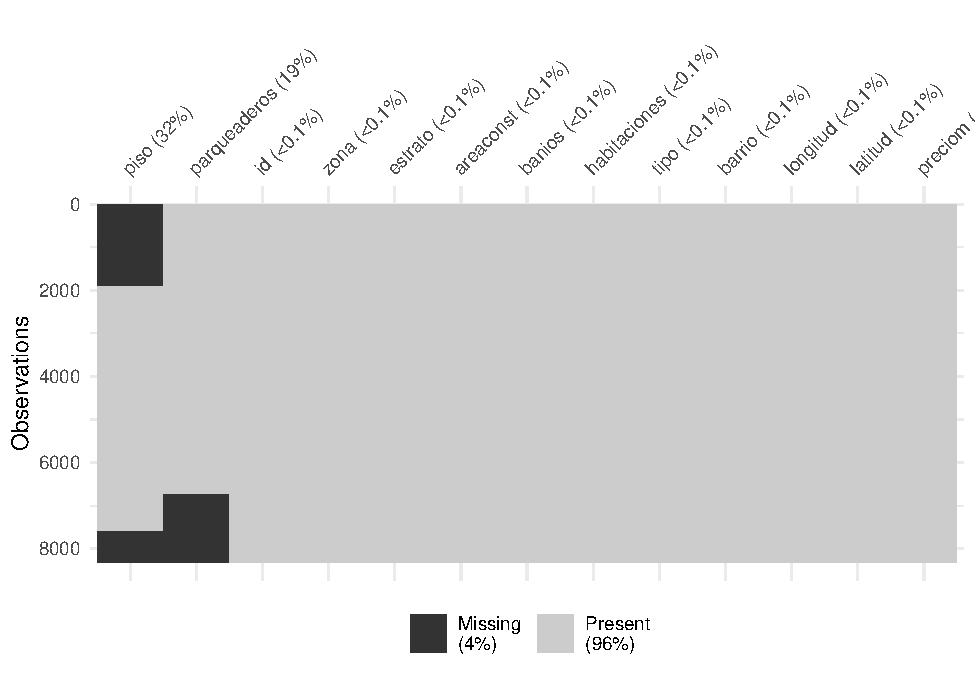
\includegraphics{A2_U2_InformeEjecutivo_files/figure-latex/unnamed-chunk-8-1.pdf}
\includegraphics{A2_U2_InformeEjecutivo_files/figure-latex/unnamed-chunk-8-2.pdf}

\begin{verbatim}
## Tabla de frecuencia de tipos de vivienda en la zona oriente:
\end{verbatim}

\begin{longtable}[]{@{}lr@{}}
\toprule\noalign{}
Var1 & Freq \\
\midrule\noalign{}
\endhead
\bottomrule\noalign{}
\endlastfoot
Casa & 289 \\
\end{longtable}

\begin{verbatim}
## Tabla de frecuencia de estratos en la zona oriente:
\end{verbatim}

\begin{longtable}[]{@{}lr@{}}
\toprule\noalign{}
Var1 & Freq \\
\midrule\noalign{}
\endhead
\bottomrule\noalign{}
\endlastfoot
3 & 282 \\
4 & 6 \\
5 & 1 \\
\end{longtable}

\begin{verbatim}
## Tabla de frecuencia de barrios en la zona oriente (ordenada por frecuencia descendente):
\end{verbatim}

\begin{longtable}[]{@{}lr@{}}
\toprule\noalign{}
Var1 & Freq \\
\midrule\noalign{}
\endhead
\bottomrule\noalign{}
\endlastfoot
alfonso lópez & 19 \\
atanasio girardot & 7 \\
20 de julio & 3 \\
antonio nariño & 2 \\
agua blanca & 1 \\
aguablanca & 1 \\
alfonso lopez & 1 \\
alfonso lópez i & 1 \\
arboleda campestre candelaria & 1 \\
autopista sur & 1 \\
\end{longtable}

Base 4 Casas Zona Oeste

Las estadísticas descriptivas de las ofertas de casas en la zona oeste
reflejan una distribución diversa en los datos. Con un total de 169
registros, se aprecia una variabilidad considerable en los atributos
considerados. Al igual que en otras zonas, se identifican valores
faltantes en algunos atributos, lo cual es coherente con la estructura
original del dataset.

En relación a los precios de las casas, se evidencia una variación
amplia, con valores que oscilan entre 135 y 1999 unidades monetarias.
Tanto la mediana como la media sugieren que la mayoría de las casas
tienen precios alrededor de 680 y 736.4 unidades monetarias,
respectivamente.

El análisis del área construida también muestra una diversidad notable,
con valores que van desde 55 hasta 1200 metros cuadrados. La mediana y
la media indican que la mayoría de las casas tienen un área construida
de alrededor de 300 y 343.2 metros cuadrados, respectivamente.

\begin{verbatim}
## Primeros 3 registros de la base de datos filtrada:
\end{verbatim}

\begin{longtable}[]{@{}
  >{\raggedleft\arraybackslash}p{(\columnwidth - 24\tabcolsep) * \real{0.0442}}
  >{\raggedright\arraybackslash}p{(\columnwidth - 24\tabcolsep) * \real{0.0973}}
  >{\raggedright\arraybackslash}p{(\columnwidth - 24\tabcolsep) * \real{0.0442}}
  >{\raggedleft\arraybackslash}p{(\columnwidth - 24\tabcolsep) * \real{0.0708}}
  >{\raggedleft\arraybackslash}p{(\columnwidth - 24\tabcolsep) * \real{0.0708}}
  >{\raggedleft\arraybackslash}p{(\columnwidth - 24\tabcolsep) * \real{0.0885}}
  >{\raggedleft\arraybackslash}p{(\columnwidth - 24\tabcolsep) * \real{0.1150}}
  >{\raggedleft\arraybackslash}p{(\columnwidth - 24\tabcolsep) * \real{0.0619}}
  >{\raggedleft\arraybackslash}p{(\columnwidth - 24\tabcolsep) * \real{0.1150}}
  >{\raggedright\arraybackslash}p{(\columnwidth - 24\tabcolsep) * \real{0.0442}}
  >{\raggedright\arraybackslash}p{(\columnwidth - 24\tabcolsep) * \real{0.0885}}
  >{\raggedleft\arraybackslash}p{(\columnwidth - 24\tabcolsep) * \real{0.0885}}
  >{\raggedleft\arraybackslash}p{(\columnwidth - 24\tabcolsep) * \real{0.0708}}@{}}
\toprule\noalign{}
\begin{minipage}[b]{\linewidth}\raggedleft
id
\end{minipage} & \begin{minipage}[b]{\linewidth}\raggedright
zona
\end{minipage} & \begin{minipage}[b]{\linewidth}\raggedright
piso
\end{minipage} & \begin{minipage}[b]{\linewidth}\raggedleft
estrato
\end{minipage} & \begin{minipage}[b]{\linewidth}\raggedleft
preciom
\end{minipage} & \begin{minipage}[b]{\linewidth}\raggedleft
areaconst
\end{minipage} & \begin{minipage}[b]{\linewidth}\raggedleft
parqueaderos
\end{minipage} & \begin{minipage}[b]{\linewidth}\raggedleft
banios
\end{minipage} & \begin{minipage}[b]{\linewidth}\raggedleft
habitaciones
\end{minipage} & \begin{minipage}[b]{\linewidth}\raggedright
tipo
\end{minipage} & \begin{minipage}[b]{\linewidth}\raggedright
barrio
\end{minipage} & \begin{minipage}[b]{\linewidth}\raggedleft
longitud
\end{minipage} & \begin{minipage}[b]{\linewidth}\raggedleft
latitud
\end{minipage} \\
\midrule\noalign{}
\endhead
\bottomrule\noalign{}
\endlastfoot
6928 & Zona Oeste & 03 & 6 & 1850 & 302 & 4 & 4 & 3 & Casa & aguacatal &
-76.54600 & 3.44400 \\
7510 & Zona Oeste & 03 & 6 & 1950 & 400 & 4 & 5 & 3 & Casa & aguacatal &
-76.55000 & 3.45600 \\
7586 & Zona Oeste & 03 & 6 & 870 & 275 & 3 & 5 & 4 & Casa & aguacatal &
-76.55074 & 3.45649 \\
\end{longtable}

\begin{verbatim}
## Estadísticas descriptivas de las ofertas de casas en la zona Oeste:
\end{verbatim}

\begin{longtable}[]{@{}
  >{\raggedright\arraybackslash}p{(\columnwidth - 26\tabcolsep) * \real{0.0151}}
  >{\raggedright\arraybackslash}p{(\columnwidth - 26\tabcolsep) * \real{0.0653}}
  >{\raggedright\arraybackslash}p{(\columnwidth - 26\tabcolsep) * \real{0.0854}}
  >{\raggedright\arraybackslash}p{(\columnwidth - 26\tabcolsep) * \real{0.0854}}
  >{\raggedright\arraybackslash}p{(\columnwidth - 26\tabcolsep) * \real{0.0704}}
  >{\raggedright\arraybackslash}p{(\columnwidth - 26\tabcolsep) * \real{0.0754}}
  >{\raggedright\arraybackslash}p{(\columnwidth - 26\tabcolsep) * \real{0.0754}}
  >{\raggedright\arraybackslash}p{(\columnwidth - 26\tabcolsep) * \real{0.0704}}
  >{\raggedright\arraybackslash}p{(\columnwidth - 26\tabcolsep) * \real{0.0653}}
  >{\raggedright\arraybackslash}p{(\columnwidth - 26\tabcolsep) * \real{0.0754}}
  >{\raggedright\arraybackslash}p{(\columnwidth - 26\tabcolsep) * \real{0.0854}}
  >{\raggedright\arraybackslash}p{(\columnwidth - 26\tabcolsep) * \real{0.0854}}
  >{\raggedright\arraybackslash}p{(\columnwidth - 26\tabcolsep) * \real{0.0754}}
  >{\raggedright\arraybackslash}p{(\columnwidth - 26\tabcolsep) * \real{0.0704}}@{}}
\toprule\noalign{}
\begin{minipage}[b]{\linewidth}\raggedright
\end{minipage} & \begin{minipage}[b]{\linewidth}\raggedright
id
\end{minipage} & \begin{minipage}[b]{\linewidth}\raggedright
zona
\end{minipage} & \begin{minipage}[b]{\linewidth}\raggedright
piso
\end{minipage} & \begin{minipage}[b]{\linewidth}\raggedright
estrato
\end{minipage} & \begin{minipage}[b]{\linewidth}\raggedright
preciom
\end{minipage} & \begin{minipage}[b]{\linewidth}\raggedright
areaconst
\end{minipage} & \begin{minipage}[b]{\linewidth}\raggedright
parqueaderos
\end{minipage} & \begin{minipage}[b]{\linewidth}\raggedright
banios
\end{minipage} & \begin{minipage}[b]{\linewidth}\raggedright
habitaciones
\end{minipage} & \begin{minipage}[b]{\linewidth}\raggedright
tipo
\end{minipage} & \begin{minipage}[b]{\linewidth}\raggedright
barrio
\end{minipage} & \begin{minipage}[b]{\linewidth}\raggedright
longitud
\end{minipage} & \begin{minipage}[b]{\linewidth}\raggedright
latitud
\end{minipage} \\
\midrule\noalign{}
\endhead
\bottomrule\noalign{}
\endlastfoot
& Min. : 2 & Length:169 & Length:169 & Min. :3.000 & Min. : 135.0 & Min.
: 55.0 & Min. :1.000 & Min. :0.00 & Min. : 0.000 & Length:169 &
Length:169 & Min. :-76.57 & Min. :3.398 \\
& 1st Qu.:5836 & Class :character & Class :character & 1st Qu.:4.000 &
1st Qu.: 430.0 & 1st Qu.: 233.0 & 1st Qu.:1.000 & 1st Qu.:3.00 & 1st
Qu.: 4.000 & Class :character & Class :character & 1st Qu.:-76.55 & 1st
Qu.:3.437 \\
& Median :6725 & Mode :character & Mode :character & Median :5.000 &
Median : 680.0 & Median : 300.0 & Median :2.000 & Median :4.00 & Median
: 4.000 & Mode :character & Mode :character & Median :-76.54 & Median
:3.444 \\
& Mean :6235 & NA & NA & Mean :4.899 & Mean : 736.4 & Mean : 343.2 &
Mean :2.311 & Mean :4.26 & Mean : 4.645 & NA & NA & Mean :-76.54 & Mean
:3.443 \\
& 3rd Qu.:7332 & NA & NA & 3rd Qu.:6.000 & 3rd Qu.: 930.0 & 3rd Qu.:
435.0 & 3rd Qu.:3.000 & 3rd Qu.:5.00 & 3rd Qu.: 5.000 & NA & NA & 3rd
Qu.:-76.54 & 3rd Qu.:3.451 \\
& Max. :8311 & NA & NA & Max. :6.000 & Max. :1999.0 & Max. :1200.0 &
Max. :7.000 & Max. :9.00 & Max. :10.000 & NA & NA & Max. :-76.46 & Max.
:3.494 \\
& NA & NA & NA & NA & NA & NA & NA's :37 & NA & NA & NA & NA & NA &
NA \\
\end{longtable}

El gráfico de dispersión para la Zona Oeste muestra una correlación
positiva moderada entre el precio y el área construida, con un
coeficiente de correlación de 0.59. Esto indica una relación directa,
pero no determinante, entre ambas variables. La línea de tendencia
sugiere un aumento promedio de 0.95 millones de pesos por cada metro
cuadrado adicional, pero la considerable dispersión de los puntos
alrededor de la línea refleja una variación notable en los precios.

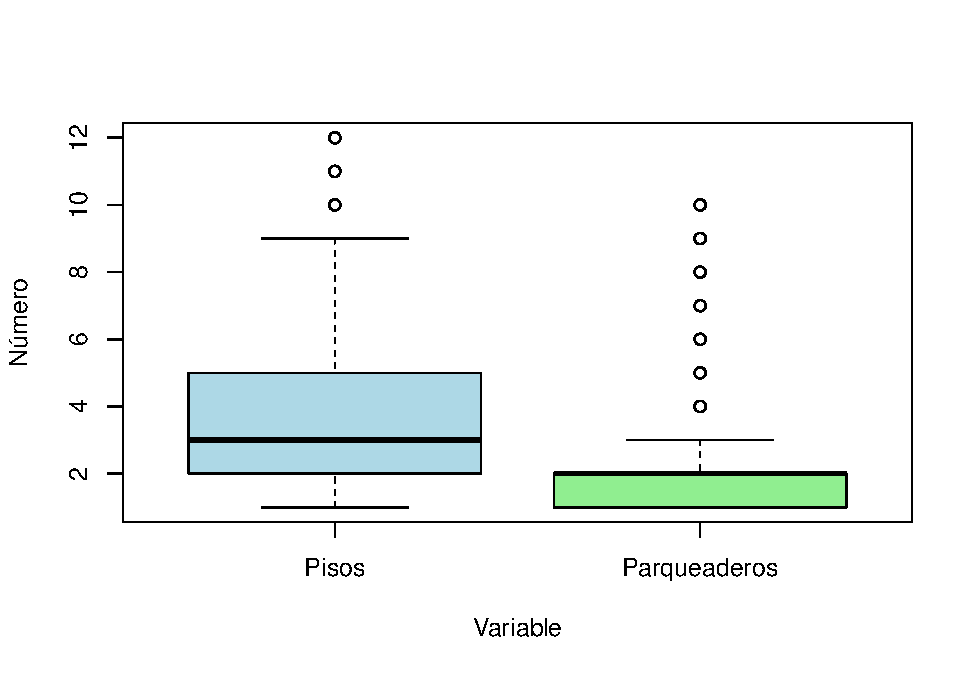
\includegraphics{A2_U2_InformeEjecutivo_files/figure-latex/unnamed-chunk-10-1.pdf}
\includegraphics{A2_U2_InformeEjecutivo_files/figure-latex/unnamed-chunk-10-2.pdf}

\begin{verbatim}
## Tabla de frecuencia de tipos de vivienda en la zona Oeste:
\end{verbatim}

\begin{longtable}[]{@{}lr@{}}
\toprule\noalign{}
Var1 & Freq \\
\midrule\noalign{}
\endhead
\bottomrule\noalign{}
\endlastfoot
Casa & 169 \\
\end{longtable}

\begin{verbatim}
## Tabla de frecuencia de estratos en la zona Oeste:
\end{verbatim}

\begin{longtable}[]{@{}lr@{}}
\toprule\noalign{}
Var1 & Freq \\
\midrule\noalign{}
\endhead
\bottomrule\noalign{}
\endlastfoot
3 & 25 \\
4 & 26 \\
5 & 59 \\
6 & 59 \\
\end{longtable}

\begin{verbatim}
## Tabla de frecuencia de barrios en la zona oeste (ordenada por frecuencia descendente):
\end{verbatim}

\begin{longtable}[]{@{}lr@{}}
\toprule\noalign{}
Var1 & Freq \\
\midrule\noalign{}
\endhead
\bottomrule\noalign{}
\endlastfoot
aguacatal & 11 \\
cristales & 10 \\
bella suiza & 7 \\
bellavista & 7 \\
el peñon & 4 \\
altos de guadalupe & 1 \\
bella suiza alta & 1 \\
el nacional & 1 \\
juanamb√∫ & 1 \\
la cascada & 1 \\
\end{longtable}

Base 5 Casas Zona Centro

Las estadísticas descriptivas de las ofertas de casas en la zona centro
revelan una distribución diversificada en los datos. Con un total de 100
registros, se destaca una variabilidad significativa en los atributos
considerados. Al igual que en otras zonas, se encuentran valores
faltantes en algunos atributos, lo cual es coherente con la estructura
original del dataset.

En cuanto a los precios de las casas, se observa una variación
considerable, con valores que van desde 148 hasta 1100 unidades
monetarias. Tanto la mediana como la media sugieren que la mayoría de
las casas tienen precios alrededor de 310 y 339.2 unidades monetarias,
respectivamente.

El análisis del área construida también muestra una diversidad
significativa, con valores que van desde 74 hasta 750 metros cuadrados.
La mediana y la media indican que la mayoría de las casas tienen un área
construida de alrededor de 200 y 217.8 metros cuadrados,
respectivamente.

\begin{verbatim}
## Primeros 3 registros de la base de datos filtrada:
\end{verbatim}

\begin{longtable}[]{@{}
  >{\raggedleft\arraybackslash}p{(\columnwidth - 24\tabcolsep) * \real{0.0446}}
  >{\raggedright\arraybackslash}p{(\columnwidth - 24\tabcolsep) * \real{0.1071}}
  >{\raggedright\arraybackslash}p{(\columnwidth - 24\tabcolsep) * \real{0.0446}}
  >{\raggedleft\arraybackslash}p{(\columnwidth - 24\tabcolsep) * \real{0.0714}}
  >{\raggedleft\arraybackslash}p{(\columnwidth - 24\tabcolsep) * \real{0.0714}}
  >{\raggedleft\arraybackslash}p{(\columnwidth - 24\tabcolsep) * \real{0.0893}}
  >{\raggedleft\arraybackslash}p{(\columnwidth - 24\tabcolsep) * \real{0.1161}}
  >{\raggedleft\arraybackslash}p{(\columnwidth - 24\tabcolsep) * \real{0.0625}}
  >{\raggedleft\arraybackslash}p{(\columnwidth - 24\tabcolsep) * \real{0.1161}}
  >{\raggedright\arraybackslash}p{(\columnwidth - 24\tabcolsep) * \real{0.0446}}
  >{\raggedright\arraybackslash}p{(\columnwidth - 24\tabcolsep) * \real{0.0714}}
  >{\raggedleft\arraybackslash}p{(\columnwidth - 24\tabcolsep) * \real{0.0893}}
  >{\raggedleft\arraybackslash}p{(\columnwidth - 24\tabcolsep) * \real{0.0714}}@{}}
\toprule\noalign{}
\begin{minipage}[b]{\linewidth}\raggedleft
id
\end{minipage} & \begin{minipage}[b]{\linewidth}\raggedright
zona
\end{minipage} & \begin{minipage}[b]{\linewidth}\raggedright
piso
\end{minipage} & \begin{minipage}[b]{\linewidth}\raggedleft
estrato
\end{minipage} & \begin{minipage}[b]{\linewidth}\raggedleft
preciom
\end{minipage} & \begin{minipage}[b]{\linewidth}\raggedleft
areaconst
\end{minipage} & \begin{minipage}[b]{\linewidth}\raggedleft
parqueaderos
\end{minipage} & \begin{minipage}[b]{\linewidth}\raggedleft
banios
\end{minipage} & \begin{minipage}[b]{\linewidth}\raggedleft
habitaciones
\end{minipage} & \begin{minipage}[b]{\linewidth}\raggedright
tipo
\end{minipage} & \begin{minipage}[b]{\linewidth}\raggedright
barrio
\end{minipage} & \begin{minipage}[b]{\linewidth}\raggedleft
longitud
\end{minipage} & \begin{minipage}[b]{\linewidth}\raggedleft
latitud
\end{minipage} \\
\midrule\noalign{}
\endhead
\bottomrule\noalign{}
\endlastfoot
5298 & Zona Centro & 01 & 3 & 650 & 240 & 2 & 4 & 4 & Casa & alameda &
-76.53564 & 3.43521 \\
5107 & Zona Centro & 02 & 4 & 400 & 460 & NA & 5 & 7 & Casa & alameda &
-76.53471 & 3.43627 \\
5117 & Zona Centro & 02 & 3 & 380 & 290 & NA & 4 & 8 & Casa & alameda &
-76.53481 & 3.43712 \\
\end{longtable}

\begin{verbatim}
## Estadísticas descriptivas de las ofertas de casas en la zona Centro:
\end{verbatim}

\begin{longtable}[]{@{}
  >{\raggedright\arraybackslash}p{(\columnwidth - 26\tabcolsep) * \real{0.0153}}
  >{\raggedright\arraybackslash}p{(\columnwidth - 26\tabcolsep) * \real{0.0663}}
  >{\raggedright\arraybackslash}p{(\columnwidth - 26\tabcolsep) * \real{0.0867}}
  >{\raggedright\arraybackslash}p{(\columnwidth - 26\tabcolsep) * \real{0.0867}}
  >{\raggedright\arraybackslash}p{(\columnwidth - 26\tabcolsep) * \real{0.0663}}
  >{\raggedright\arraybackslash}p{(\columnwidth - 26\tabcolsep) * \real{0.0765}}
  >{\raggedright\arraybackslash}p{(\columnwidth - 26\tabcolsep) * \real{0.0714}}
  >{\raggedright\arraybackslash}p{(\columnwidth - 26\tabcolsep) * \real{0.0714}}
  >{\raggedright\arraybackslash}p{(\columnwidth - 26\tabcolsep) * \real{0.0663}}
  >{\raggedright\arraybackslash}p{(\columnwidth - 26\tabcolsep) * \real{0.0714}}
  >{\raggedright\arraybackslash}p{(\columnwidth - 26\tabcolsep) * \real{0.0867}}
  >{\raggedright\arraybackslash}p{(\columnwidth - 26\tabcolsep) * \real{0.0867}}
  >{\raggedright\arraybackslash}p{(\columnwidth - 26\tabcolsep) * \real{0.0765}}
  >{\raggedright\arraybackslash}p{(\columnwidth - 26\tabcolsep) * \real{0.0714}}@{}}
\toprule\noalign{}
\begin{minipage}[b]{\linewidth}\raggedright
\end{minipage} & \begin{minipage}[b]{\linewidth}\raggedright
id
\end{minipage} & \begin{minipage}[b]{\linewidth}\raggedright
zona
\end{minipage} & \begin{minipage}[b]{\linewidth}\raggedright
piso
\end{minipage} & \begin{minipage}[b]{\linewidth}\raggedright
estrato
\end{minipage} & \begin{minipage}[b]{\linewidth}\raggedright
preciom
\end{minipage} & \begin{minipage}[b]{\linewidth}\raggedright
areaconst
\end{minipage} & \begin{minipage}[b]{\linewidth}\raggedright
parqueaderos
\end{minipage} & \begin{minipage}[b]{\linewidth}\raggedright
banios
\end{minipage} & \begin{minipage}[b]{\linewidth}\raggedright
habitaciones
\end{minipage} & \begin{minipage}[b]{\linewidth}\raggedright
tipo
\end{minipage} & \begin{minipage}[b]{\linewidth}\raggedright
barrio
\end{minipage} & \begin{minipage}[b]{\linewidth}\raggedright
longitud
\end{minipage} & \begin{minipage}[b]{\linewidth}\raggedright
latitud
\end{minipage} \\
\midrule\noalign{}
\endhead
\bottomrule\noalign{}
\endlastfoot
& Min. : 572 & Length:100 & Length:100 & Min. :3.00 & Min. : 148.0 &
Min. : 74.0 & Min. :1.000 & Min. :0.00 & Min. : 0.00 & Length:100 &
Length:100 & Min. :-76.54 & Min. :3.398 \\
& 1st Qu.:2976 & Class :character & Class :character & 1st Qu.:3.00 &
1st Qu.: 238.8 & 1st Qu.:146.5 & 1st Qu.:1.000 & 1st Qu.:2.00 & 1st Qu.:
3.00 & Class :character & Class :character & 1st Qu.:-76.53 & 1st
Qu.:3.436 \\
& Median :3739 & Mode :character & Mode :character & Median :3.00 &
Median : 310.0 & Median :200.0 & Median :1.000 & Median :3.00 & Median :
5.00 & Mode :character & Mode :character & Median :-76.53 & Median
:3.439 \\
& Mean :3816 & NA & NA & Mean :3.12 & Mean : 339.2 & Mean :217.8 & Mean
:1.481 & Mean :3.01 & Mean : 5.11 & NA & NA & Mean :-76.53 & Mean
:3.440 \\
& 3rd Qu.:4765 & NA & NA & 3rd Qu.:3.00 & 3rd Qu.: 382.5 & 3rd Qu.:265.5
& 3rd Qu.:1.750 & 3rd Qu.:4.00 & 3rd Qu.: 7.00 & NA & NA & 3rd
Qu.:-76.52 & 3rd Qu.:3.444 \\
& Max. :6662 & NA & NA & Max. :6.00 & Max. :1100.0 & Max. :750.0 & Max.
:6.000 & Max. :9.00 & Max. :10.00 & NA & NA & Max. :-76.50 & Max.
:3.477 \\
& NA & NA & NA & NA & NA & NA & NA's :46 & NA & NA & NA & NA & NA &
NA \\
\end{longtable}

El gráfico de dispersión para la Zona Centro revela una correlación
positiva moderada entre el precio y el área construida, con un
coeficiente de correlación de 0.53. Si bien existe una relación directa
entre ambas variables, la influencia del área construida sobre el precio
es menor que en otras zonas. La línea de tendencia indica un aumento
promedio de 0.85 millones de pesos por cada metro cuadrado adicional,
pero la notable dispersión de los puntos alrededor de la línea refleja
una variabilidad considerable en los precios.

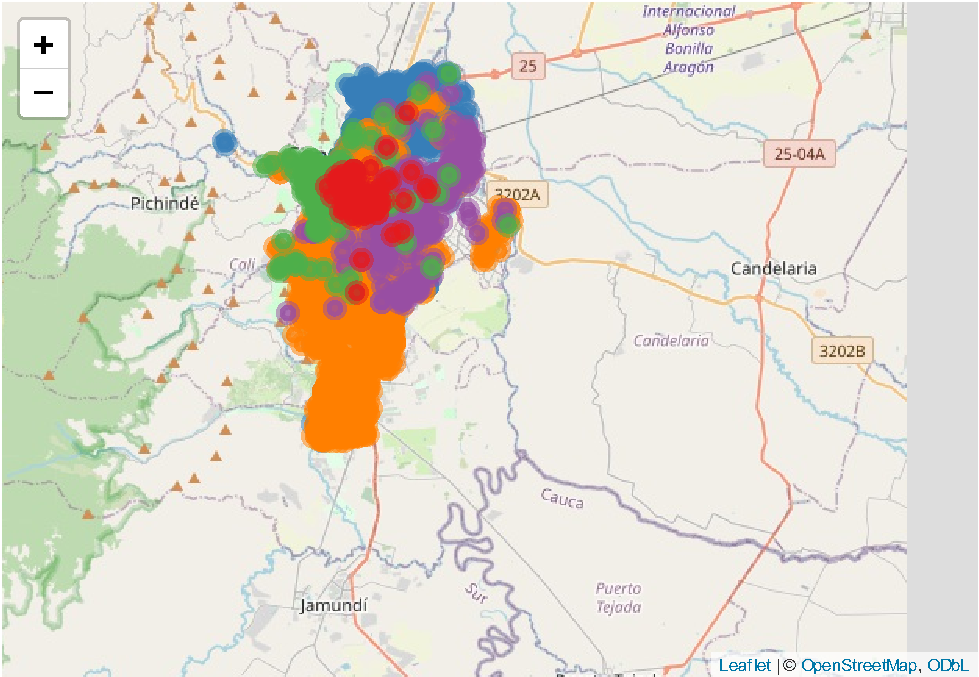
\includegraphics{A2_U2_InformeEjecutivo_files/figure-latex/unnamed-chunk-12-1.pdf}
\includegraphics{A2_U2_InformeEjecutivo_files/figure-latex/unnamed-chunk-12-2.pdf}

\begin{verbatim}
## Tabla de frecuencia de tipos de vivienda en la zona Centro:
\end{verbatim}

\begin{longtable}[]{@{}lr@{}}
\toprule\noalign{}
Var1 & Freq \\
\midrule\noalign{}
\endhead
\bottomrule\noalign{}
\endlastfoot
Casa & 100 \\
\end{longtable}

\begin{verbatim}
## Tabla de frecuencia de estratos en la zona Centro:
\end{verbatim}

\begin{longtable}[]{@{}lr@{}}
\toprule\noalign{}
Var1 & Freq \\
\midrule\noalign{}
\endhead
\bottomrule\noalign{}
\endlastfoot
3 & 91 \\
4 & 7 \\
5 & 1 \\
6 & 1 \\
\end{longtable}

\begin{verbatim}
## Tabla de frecuencia de barrios en la zona oriente (ordenada por frecuencia descendente):
\end{verbatim}

\begin{longtable}[]{@{}lr@{}}
\toprule\noalign{}
Var1 & Freq \\
\midrule\noalign{}
\endhead
\bottomrule\noalign{}
\endlastfoot
aranjuez & 14 \\
bretaña & 11 \\
alameda & 9 \\
centro & 3 \\
belalcazar & 2 \\
benjamín herrera & 2 \\
barrio obrero & 1 \\
Belalcazar & 1 \\
colseguros & 1 \\
el troncal & 1 \\
\end{longtable}

Momento de discusión

En el siguiente mapa se puede observar a una sola vista como se
encuentra la distribución de casas según la zona registrada en el
dataset, es importante destacar que se logra identificar que existen
barrios que según sus coordenadas comparten la misma zona, esto puede
deberse a errores humanos en el ingreso de longitud y latitud o en la
asignación de la variable barrio en el sistema de información que se
diseñó para la captura de los datos.

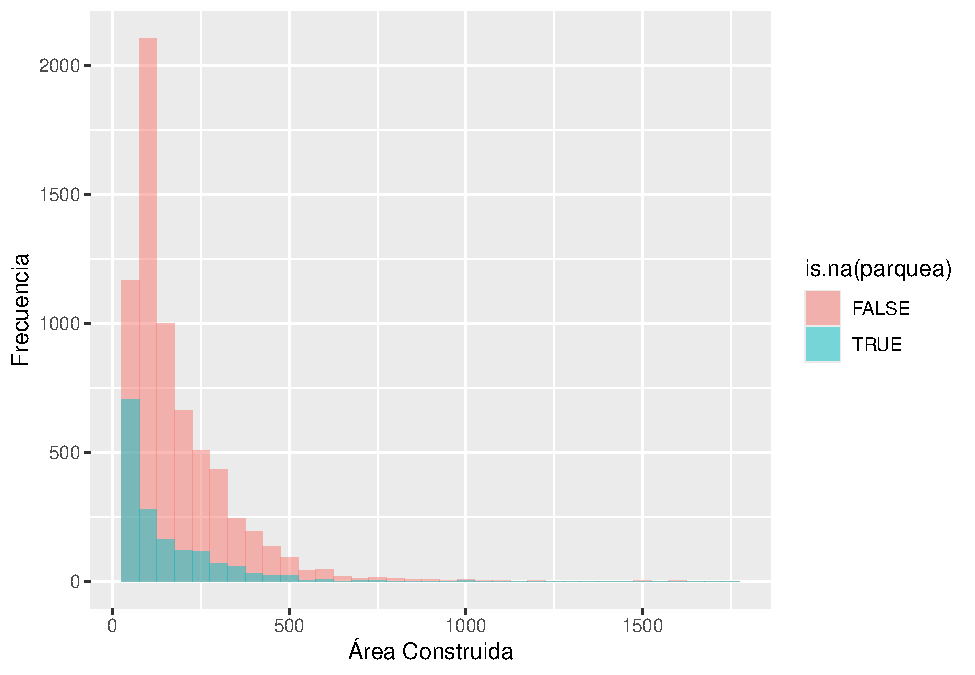
\includegraphics{A2_U2_InformeEjecutivo_files/figure-latex/unnamed-chunk-13-1.pdf}

\subsection{2. EDA}\label{eda}

Correlación de la variable precio de la casa en función de: área
construida, estrato, numero de baños, numero de habitaciones y zona
donde se ubica la vivienda

En este apartado teniendo en cuenta el EDA realizado como resultado del
análisis de correlación entre la variable respuesta (preciom) del tipo
de vivienda Casa y las variables predictoras (areaconst, estrato,
banios, habitaciones y zona) se grafican a continuación 2 modelos de
graficas:

\begin{itemize}
\item
  Dispersión: Este tipo de gráfico se utiliza para visualizar la
  relación entre dos variables cuantitativas, como el precio y el área
  construida, el precio y el estrato, el precio y el número de baños, y
  el precio y el número de habitaciones. Cada punto en el gráfico
  representa una observación en el conjunto de datos. La posición de
  cada punto en los ejes x e y representa los valores de las dos
  variables.
\item
  Caja de bigotes: Este tipo de gráfico se utiliza para visualizar la
  distribución de una variable numérica en diferentes niveles de una
  variable categórica. En este caso, se utiliza para visualizar la
  distribución de los precios (variable respuesta) en cada zona
  (variable categórica).
\end{itemize}

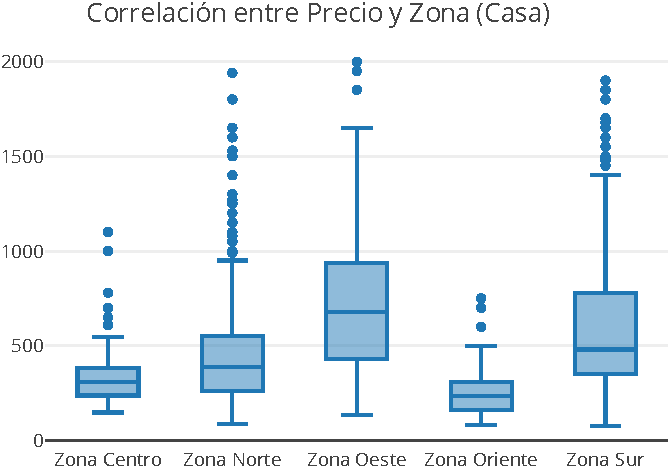
\includegraphics{A2_U2_InformeEjecutivo_files/figure-latex/unnamed-chunk-15-1.pdf}
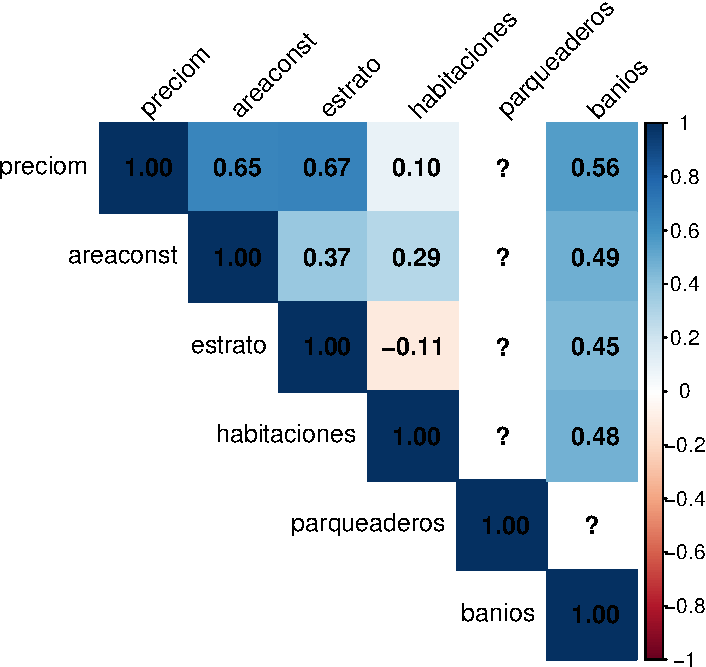
\includegraphics{A2_U2_InformeEjecutivo_files/figure-latex/unnamed-chunk-15-2.pdf}
\includegraphics{A2_U2_InformeEjecutivo_files/figure-latex/unnamed-chunk-15-3.pdf}
\includegraphics{A2_U2_InformeEjecutivo_files/figure-latex/unnamed-chunk-15-4.pdf}

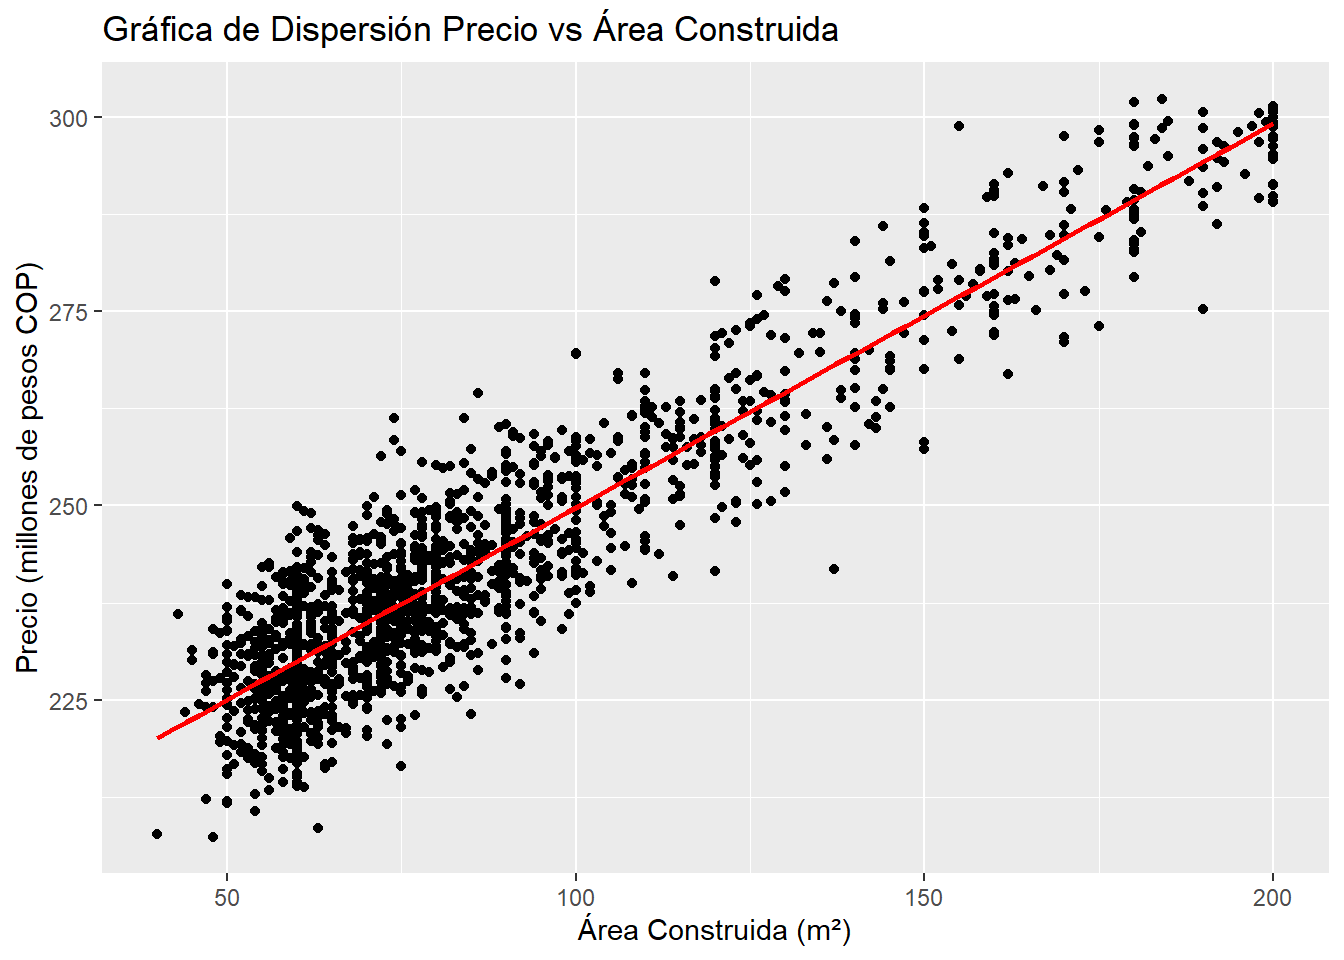
\includegraphics{A2_U2_InformeEjecutivo_files/figure-latex/unnamed-chunk-16-1.pdf}

\begin{verbatim}
##                 preciom areaconst    estrato habitaciones parqueaderos
## preciom      1.00000000 0.6529498  0.6658021   0.09683573           NA
## areaconst    0.65294983 1.0000000  0.3701747   0.28660204           NA
## estrato      0.66580209 0.3701747  1.0000000  -0.11405430           NA
## habitaciones 0.09683573 0.2866020 -0.1140543   1.00000000           NA
## parqueaderos         NA        NA         NA           NA            1
## banios       0.55810021 0.4871721  0.4488832   0.47574058           NA
##                 banios
## preciom      0.5581002
## areaconst    0.4871721
## estrato      0.4488832
## habitaciones 0.4757406
## parqueaderos        NA
## banios       1.0000000
\end{verbatim}

\includegraphics{A2_U2_InformeEjecutivo_files/figure-latex/unnamed-chunk-16-2.pdf}

La correlación más alta con ``preciom'' es con la variable ``estrato''
(0.6658), seguida por ``areaconst'' (0.6529) y ``banios'' (0.5581). Esto
indica que hay una correlación positiva moderada a fuerte entre el
precio de la vivienda y estas características.

\subsection{3. Estimación de un modelo de regresión lineal
múltiple}\label{estimaciuxf3n-de-un-modelo-de-regresiuxf3n-lineal-muxfaltiple}

\begin{verbatim}
## 
## Call:
## lm(formula = preciom ~ areaconst + estrato + habitaciones + parqueaderos + 
##     banios, data = vivienda_casa)
## 
## Residuals:
##      Min       1Q   Median       3Q      Max 
## -1190.80  -114.52   -25.94    74.59   986.16 
## 
## Coefficients:
##                Estimate Std. Error t value Pr(>|t|)    
## (Intercept)  -413.87536   25.58852 -16.174  < 2e-16 ***
## areaconst       0.74227    0.02941  25.235  < 2e-16 ***
## estrato       116.07109    5.26618  22.041  < 2e-16 ***
## habitaciones  -14.74995    3.18137  -4.636 3.73e-06 ***
## parqueaderos   64.29943    3.47719  18.492  < 2e-16 ***
## banios         39.03498    4.05083   9.636  < 2e-16 ***
## ---
## Signif. codes:  0 '***' 0.001 '**' 0.01 '*' 0.05 '.' 0.1 ' ' 1
## 
## Residual standard error: 205.2 on 2480 degrees of freedom
##   (733 observations deleted due to missingness)
## Multiple R-squared:  0.6834, Adjusted R-squared:  0.6828 
## F-statistic:  1071 on 5 and 2480 DF,  p-value: < 2.2e-16
\end{verbatim}

\begin{verbatim}
## [1] 0.6833953
\end{verbatim}

Los resultados de la estimación del modelo de regresión lineal múltiple
son los siguientes:

Interpretación de los coeficientes

:

Intercepto: El coeficiente del intercepto es -413.87536. Esto significa
que, cuando todas las demás variables son cero, el precio estimado de
una vivienda es de -413.87536 unidades monetarias. Sin embargo, dado que
este valor no tiene una interpretación realista en este contexto, no se
le da mucha importancia en la interpretación.

Área Construida: El coeficiente para el área construida es 0.74227. Esto
indica que, manteniendo constantes todas las demás variables, por cada
unidad adicional de área construida, el precio estimado de la vivienda
aumenta en 0.74227 unidades monetarias.

Estrato: El coeficiente para el estrato es 116.07109. Esto sugiere que,
manteniendo constantes todas las demás variables, el precio estimado de
la vivienda aumenta en 116.07109 unidades monetarias por cada incremento
de una unidad en el estrato.

Número de Cuartos: El coeficiente para el número de habitaciones es
-14.74995. Esto indica que, manteniendo constantes todas las demás
variables, por cada incremento de una unidad en el número de
habitaciones, el precio estimado de la vivienda disminuye en 14.74995
unidades monetarias.

Número de Parqueaderos: El coeficiente para el número de parqueaderos es
64.29943. Esto sugiere que, manteniendo constantes todas las demás
variables, por cada unidad adicional de parqueaderos, el precio estimado
de la vivienda aumenta en 64.29943 unidades monetarias.

Número de Baños: El coeficiente para el número de baños es 39.03498.
Esto indica que, manteniendo constantes todas las demás variables, por
cada unidad adicional de baños, el precio estimado de la vivienda
aumenta en 39.03498 unidades monetarias.

Gráfico de residuos vs.~valores ajustados

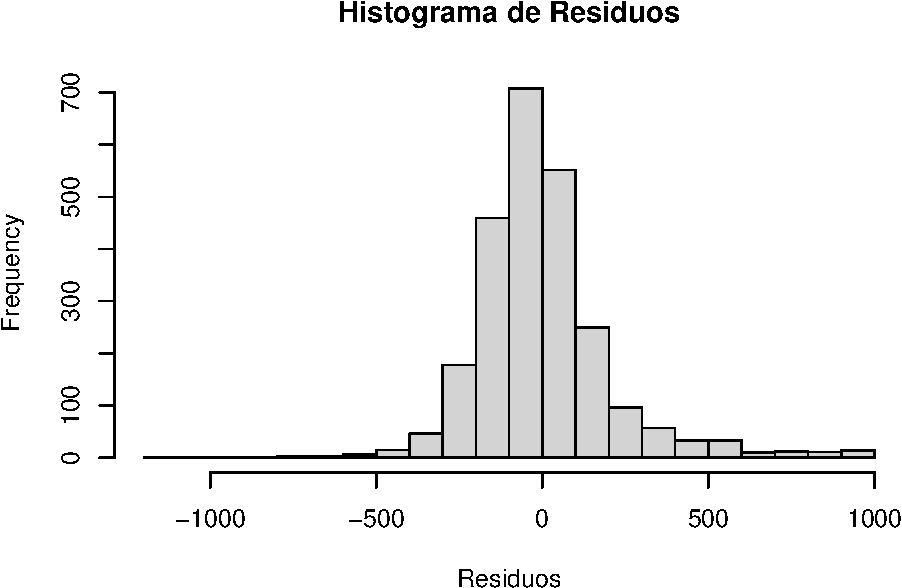
\includegraphics{A2_U2_InformeEjecutivo_files/figure-latex/unnamed-chunk-18-1.pdf}

Gráfico de distribución de los residuos

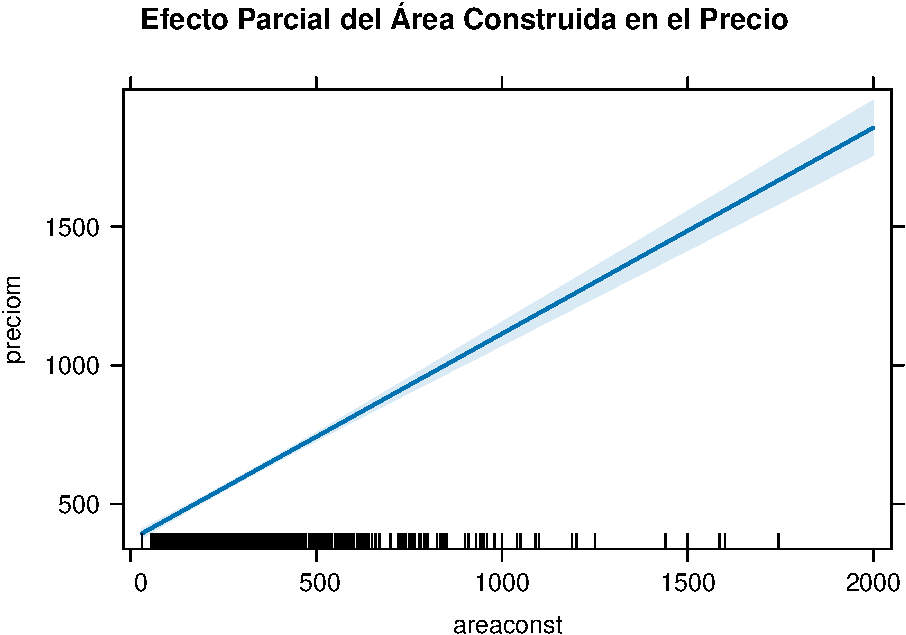
\includegraphics{A2_U2_InformeEjecutivo_files/figure-latex/unnamed-chunk-19-1.pdf}
\includegraphics{A2_U2_InformeEjecutivo_files/figure-latex/unnamed-chunk-19-2.pdf}

Gráfico de efectos parciales

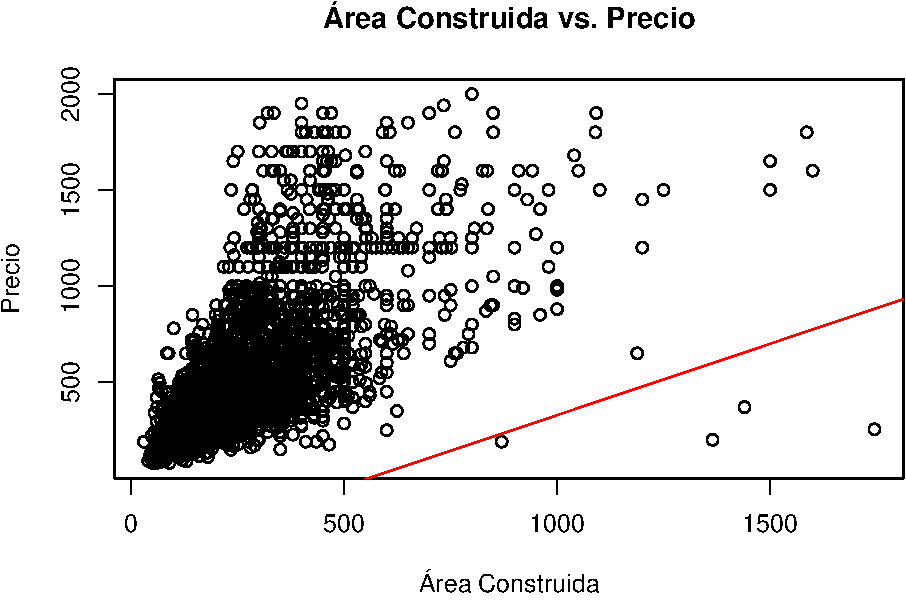
\includegraphics{A2_U2_InformeEjecutivo_files/figure-latex/unnamed-chunk-20-1.pdf}

Gráficos de dispersión con línea de regresión

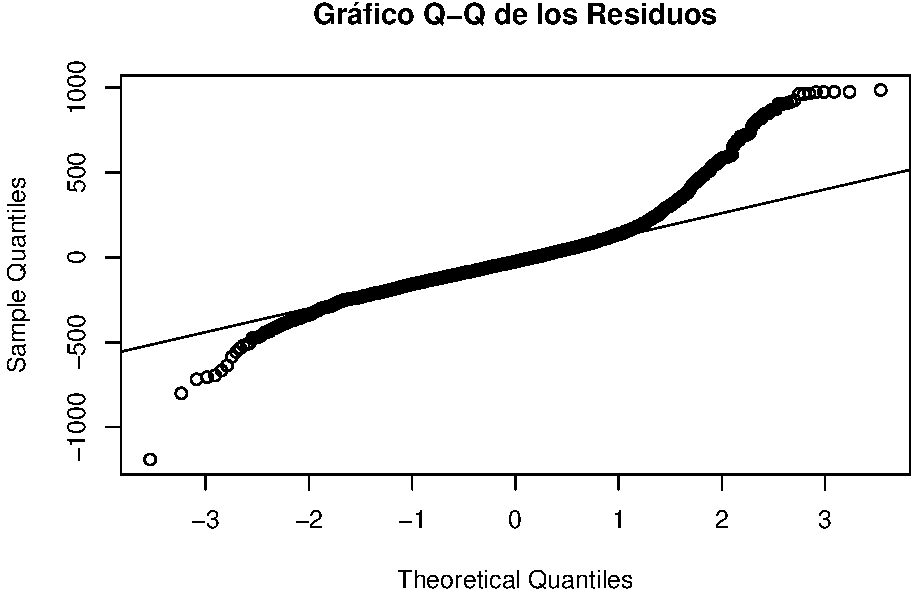
\includegraphics{A2_U2_InformeEjecutivo_files/figure-latex/unnamed-chunk-21-1.pdf}

Interpretación del coeficiente R\^{}2:

El coeficiente de determinación (R\^{}2) es aproximadamente 0.6834. Esto
significa que alrededor del 68.34\% de la variabilidad en el precio de
la vivienda puede ser explicada por las variables independientes
incluidas en el modelo. Esto indica un buen ajuste del modelo a los
datos observados.

Discusión sobre el ajuste del modelo e implicaciones: Dado que el
coeficiente de determinación es relativamente alto, sugiere que el
modelo de regresión lineal múltiple es capaz de explicar una proporción
significativa de la variabilidad en el precio de la vivienda utilizando
las variables incluidas. Sin embargo, siempre hay margen para mejorar el
modelo. Para ello, podríamos considerar la inclusión de variables
adicionales relevantes, como la ubicación geográfica, la antigüedad de
la propiedad o características específicas del vecindario, que podrían
mejorar la capacidad predictiva del modelo y explicar aún más la
variabilidad en los precios de las propiedades. Además, podríamos
explorar posibles transformaciones en las variables existentes o
técnicas de modelado más avanzadas para mejorar aún más la precisión del
modelo.

\subsection{4. Validación de
supuestos}\label{validaciuxf3n-de-supuestos}

Esta sección tiene como objetivo realizar pruebas para validar dos
supuestos importantes en el análisis de regresión lineal:

Normalidad de los residuos: En donde la prueba de Shapiro-Wilk pretende
evaluar si los residuos del modelo siguen una distribución normal. Esto
es importante porque el análisis de regresión lineal asume que los
errores (residuos) siguen una distribución normal. Si los residuos no se
distribuyen normalmente, podría indicar que el modelo no está capturando
completamente la estructura de los datos o que hay otros factores que no
se han tenido en cuenta.

Homocedasticidad de los residuos: En donde la prueba de Breusch-Pagan
pretende evaluar si los residuos tienen una varianza constante en
relación con las variables independientes. La homocedasticidad significa
que la varianza de los residuos es constante en todos los niveles de las
variables independientes. Si hay heterocedasticidad, es decir, la
varianza de los residuos no es constante, puede haber un problema de
modelado que afecte la precisión de las estimaciones y las pruebas de
hipótesis.

.

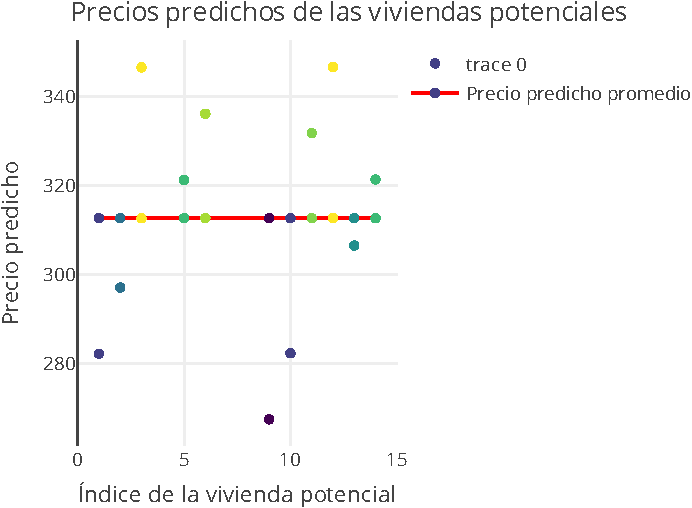
\includegraphics{A2_U2_InformeEjecutivo_files/figure-latex/unnamed-chunk-22-1.pdf}
\includegraphics{A2_U2_InformeEjecutivo_files/figure-latex/unnamed-chunk-22-2.pdf}

\begin{verbatim}
## 
##  Shapiro-Wilk normality test
## 
## data:  residuos
## W = 0.89699, p-value < 2.2e-16
\end{verbatim}

\begin{verbatim}
## 
##  studentized Breusch-Pagan test
## 
## data:  modelo_rlm_casa
## BP = 321.2, df = 5, p-value < 2.2e-16
\end{verbatim}

En conclusión, el análisis de los residuos del modelo de regresión
lineal sugiere que no se ajustan completamente a la normalidad, aunque
la desviación no es grave y el tamaño de la muestra parece ser grande.
La prueba de Shapiro-Wilk rechaza la normalidad de los residuos,
mientras que la prueba de Breusch-Pagan no encuentra evidencia de
heterocedasticidad.

\subsection{5. Predección del precio de la
vivienda}\label{predecciuxf3n-del-precio-de-la-vivienda}

\begin{verbatim}
##    index precio_predicho
## 1      1        282.1364
## 2      2        296.9818
## 3      3        346.4359
## 5      5        321.1714
## 6      6        336.0168
## 9      9        267.3865
## 10    10        282.2318
## 11    11        331.6859
## 12    12        346.5312
## 13    13        306.4215
## 14    14        321.2668
\end{verbatim}

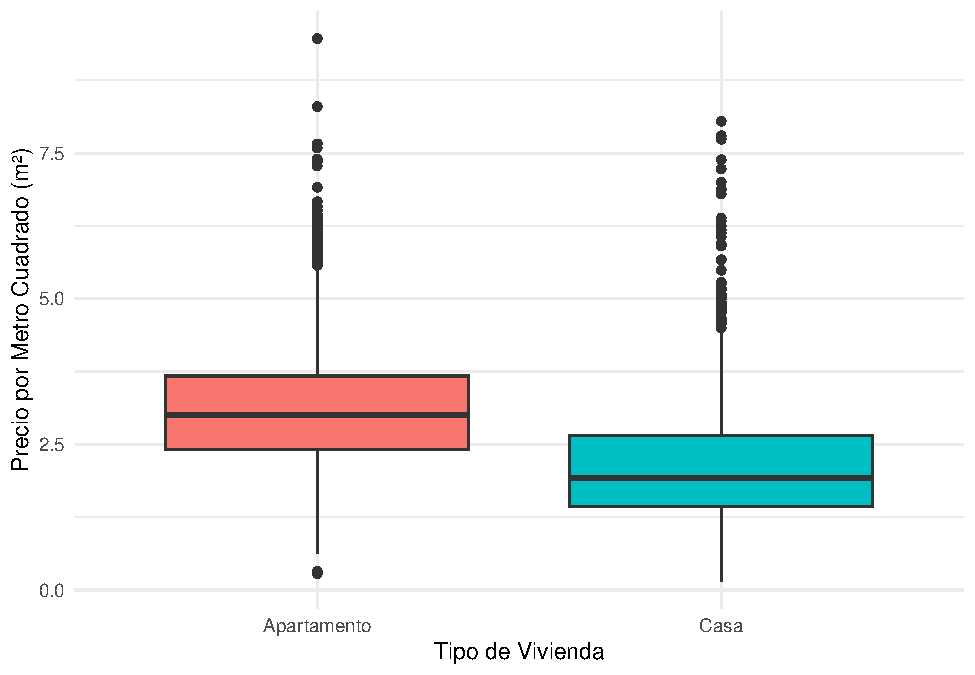
\includegraphics{A2_U2_InformeEjecutivo_files/figure-latex/unnamed-chunk-23-1.pdf}

\subsection{6. Ofertas potenciales}\label{ofertas-potenciales}

Los resultados muestran las características de las primeras cinco
viviendas potenciales que cumplen con las condiciones establecidas y
cuyo precio estimado no supera el límite del crédito preaprobado para la
nueva vivienda.

Área Construida:Las áreas construidas de estas viviendas varían entre
180 y 200 metros cuadrados. Parqueaderos: Todas las viviendas tienen al
menos un parqueadero, con una de ellas teniendo dos. Baños: La cantidad
de baños oscila entre 2 y 3. Habitaciones:** Todas las viviendas tienen
entre 3 y 4 habitaciones. Estrato: Las viviendas pertenecen a estratos
4. Zona: Todas las viviendas se encuentran en la Zona Norte. Precio
Estimado: Los precios estimados de estas viviendas varían entre 282.1364
y 346.4359 millones de pesos.

Estos resultados son útiles para presentar a Maria las primeras opciones
de viviendas potenciales que se ajustan a los criterios establecidos y
están dentro del presupuesto disponible para su compra.

\begin{verbatim}
##   areaconst parqueaderos banios habitaciones estrato       zona precio_estimado
## 1       180            1      2            3       4 Zona Norte        282.1364
## 2       200            1      2            3       4 Zona Norte        296.9818
## 3       180            2      2            3       4 Zona Norte        346.4359
## 5       180            1      3            3       4 Zona Norte        321.1714
## 6       200            1      3            3       4 Zona Norte        336.0168
\end{verbatim}

\subsection{7. Escenario de crédito pre-aprobado para tipo de vivienda
Apartamento}\label{escenario-de-cruxe9dito-pre-aprobado-para-tipo-de-vivienda-apartamento}

Segmentación por zonas

Base 1 Apartamentos Zona Norte

\begin{verbatim}
## Primeros 3 registros de la base de datos filtrada:
\end{verbatim}

\begin{longtable}[]{@{}
  >{\raggedleft\arraybackslash}p{(\columnwidth - 24\tabcolsep) * \real{0.0427}}
  >{\raggedright\arraybackslash}p{(\columnwidth - 24\tabcolsep) * \real{0.0940}}
  >{\raggedright\arraybackslash}p{(\columnwidth - 24\tabcolsep) * \real{0.0427}}
  >{\raggedleft\arraybackslash}p{(\columnwidth - 24\tabcolsep) * \real{0.0684}}
  >{\raggedleft\arraybackslash}p{(\columnwidth - 24\tabcolsep) * \real{0.0684}}
  >{\raggedleft\arraybackslash}p{(\columnwidth - 24\tabcolsep) * \real{0.0855}}
  >{\raggedleft\arraybackslash}p{(\columnwidth - 24\tabcolsep) * \real{0.1111}}
  >{\raggedleft\arraybackslash}p{(\columnwidth - 24\tabcolsep) * \real{0.0598}}
  >{\raggedleft\arraybackslash}p{(\columnwidth - 24\tabcolsep) * \real{0.1111}}
  >{\raggedright\arraybackslash}p{(\columnwidth - 24\tabcolsep) * \real{0.1026}}
  >{\raggedright\arraybackslash}p{(\columnwidth - 24\tabcolsep) * \real{0.0598}}
  >{\raggedleft\arraybackslash}p{(\columnwidth - 24\tabcolsep) * \real{0.0855}}
  >{\raggedleft\arraybackslash}p{(\columnwidth - 24\tabcolsep) * \real{0.0684}}@{}}
\toprule\noalign{}
\begin{minipage}[b]{\linewidth}\raggedleft
id
\end{minipage} & \begin{minipage}[b]{\linewidth}\raggedright
zona
\end{minipage} & \begin{minipage}[b]{\linewidth}\raggedright
piso
\end{minipage} & \begin{minipage}[b]{\linewidth}\raggedleft
estrato
\end{minipage} & \begin{minipage}[b]{\linewidth}\raggedleft
preciom
\end{minipage} & \begin{minipage}[b]{\linewidth}\raggedleft
areaconst
\end{minipage} & \begin{minipage}[b]{\linewidth}\raggedleft
parqueaderos
\end{minipage} & \begin{minipage}[b]{\linewidth}\raggedleft
banios
\end{minipage} & \begin{minipage}[b]{\linewidth}\raggedleft
habitaciones
\end{minipage} & \begin{minipage}[b]{\linewidth}\raggedright
tipo
\end{minipage} & \begin{minipage}[b]{\linewidth}\raggedright
barrio
\end{minipage} & \begin{minipage}[b]{\linewidth}\raggedleft
longitud
\end{minipage} & \begin{minipage}[b]{\linewidth}\raggedleft
latitud
\end{minipage} \\
\midrule\noalign{}
\endhead
\bottomrule\noalign{}
\endlastfoot
1212 & Zona Norte & 01 & 5 & 260 & 90 & 1 & 2 & 3 & Apartamento & acopi
& -76.51350 & 3.45891 \\
1724 & Zona Norte & 01 & 5 & 240 & 87 & 1 & 3 & 3 & Apartamento & acopi
& -76.51700 & 3.36971 \\
2326 & Zona Norte & 01 & 4 & 220 & 52 & 2 & 2 & 3 & Apartamento & acopi
& -76.51974 & 3.42627 \\
\end{longtable}

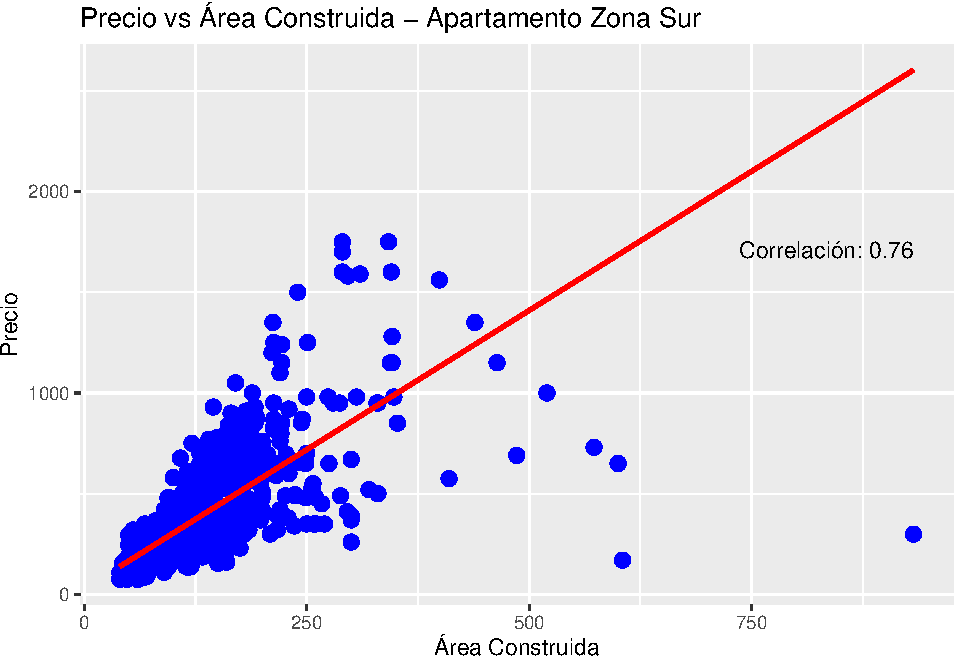
\includegraphics{A2_U2_InformeEjecutivo_files/figure-latex/unnamed-chunk-25-1.pdf}
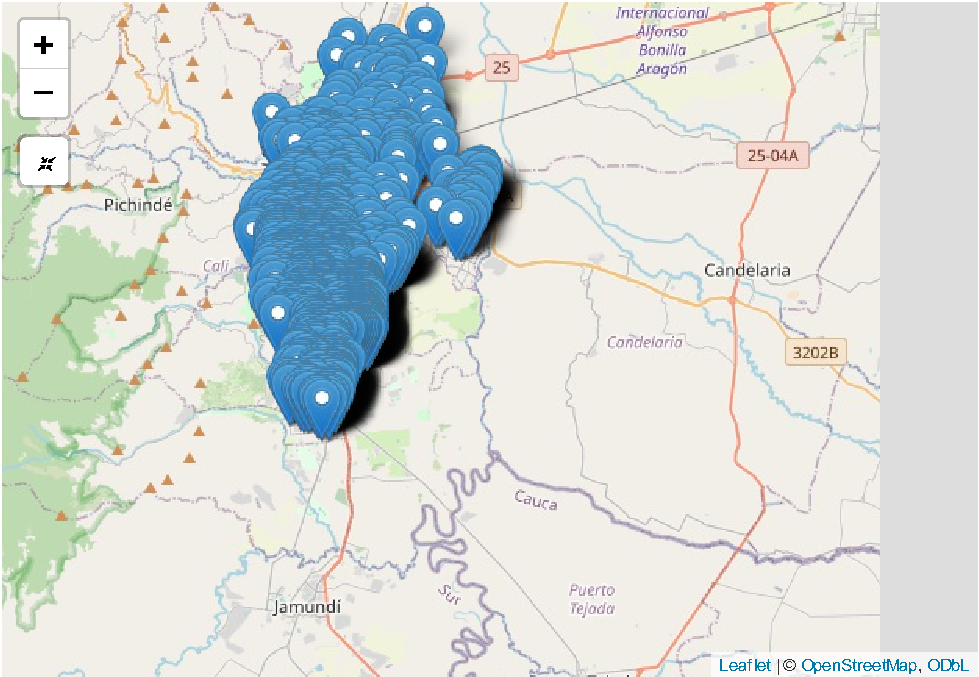
\includegraphics{A2_U2_InformeEjecutivo_files/figure-latex/unnamed-chunk-25-2.pdf}

Base 2 Apartamentos Zona Sur

\begin{verbatim}
## Primeros 3 registros de la base de datos filtrada:
\end{verbatim}

\begin{longtable}[]{@{}
  >{\raggedleft\arraybackslash}p{(\columnwidth - 24\tabcolsep) * \real{0.0420}}
  >{\raggedright\arraybackslash}p{(\columnwidth - 24\tabcolsep) * \real{0.0756}}
  >{\raggedright\arraybackslash}p{(\columnwidth - 24\tabcolsep) * \real{0.0420}}
  >{\raggedleft\arraybackslash}p{(\columnwidth - 24\tabcolsep) * \real{0.0672}}
  >{\raggedleft\arraybackslash}p{(\columnwidth - 24\tabcolsep) * \real{0.0672}}
  >{\raggedleft\arraybackslash}p{(\columnwidth - 24\tabcolsep) * \real{0.0840}}
  >{\raggedleft\arraybackslash}p{(\columnwidth - 24\tabcolsep) * \real{0.1092}}
  >{\raggedleft\arraybackslash}p{(\columnwidth - 24\tabcolsep) * \real{0.0588}}
  >{\raggedleft\arraybackslash}p{(\columnwidth - 24\tabcolsep) * \real{0.1092}}
  >{\raggedright\arraybackslash}p{(\columnwidth - 24\tabcolsep) * \real{0.1008}}
  >{\raggedright\arraybackslash}p{(\columnwidth - 24\tabcolsep) * \real{0.0924}}
  >{\raggedleft\arraybackslash}p{(\columnwidth - 24\tabcolsep) * \real{0.0840}}
  >{\raggedleft\arraybackslash}p{(\columnwidth - 24\tabcolsep) * \real{0.0672}}@{}}
\toprule\noalign{}
\begin{minipage}[b]{\linewidth}\raggedleft
id
\end{minipage} & \begin{minipage}[b]{\linewidth}\raggedright
zona
\end{minipage} & \begin{minipage}[b]{\linewidth}\raggedright
piso
\end{minipage} & \begin{minipage}[b]{\linewidth}\raggedleft
estrato
\end{minipage} & \begin{minipage}[b]{\linewidth}\raggedleft
preciom
\end{minipage} & \begin{minipage}[b]{\linewidth}\raggedleft
areaconst
\end{minipage} & \begin{minipage}[b]{\linewidth}\raggedleft
parqueaderos
\end{minipage} & \begin{minipage}[b]{\linewidth}\raggedleft
banios
\end{minipage} & \begin{minipage}[b]{\linewidth}\raggedleft
habitaciones
\end{minipage} & \begin{minipage}[b]{\linewidth}\raggedright
tipo
\end{minipage} & \begin{minipage}[b]{\linewidth}\raggedright
barrio
\end{minipage} & \begin{minipage}[b]{\linewidth}\raggedleft
longitud
\end{minipage} & \begin{minipage}[b]{\linewidth}\raggedleft
latitud
\end{minipage} \\
\midrule\noalign{}
\endhead
\bottomrule\noalign{}
\endlastfoot
5098 & Zona Sur & 05 & 4 & 290 & 96 & 1 & 2 & 3 & Apartamento & acopi &
-76.53464 & 3.44987 \\
698 & Zona Sur & 02 & 3 & 78 & 40 & 1 & 1 & 2 & Apartamento & aguablanca
& -76.50100 & 3.40000 \\
8199 & Zona Sur & NA & 6 & 875 & 194 & 2 & 5 & 3 & Apartamento &
aguacatal & -76.55700 & 3.45900 \\
\end{longtable}

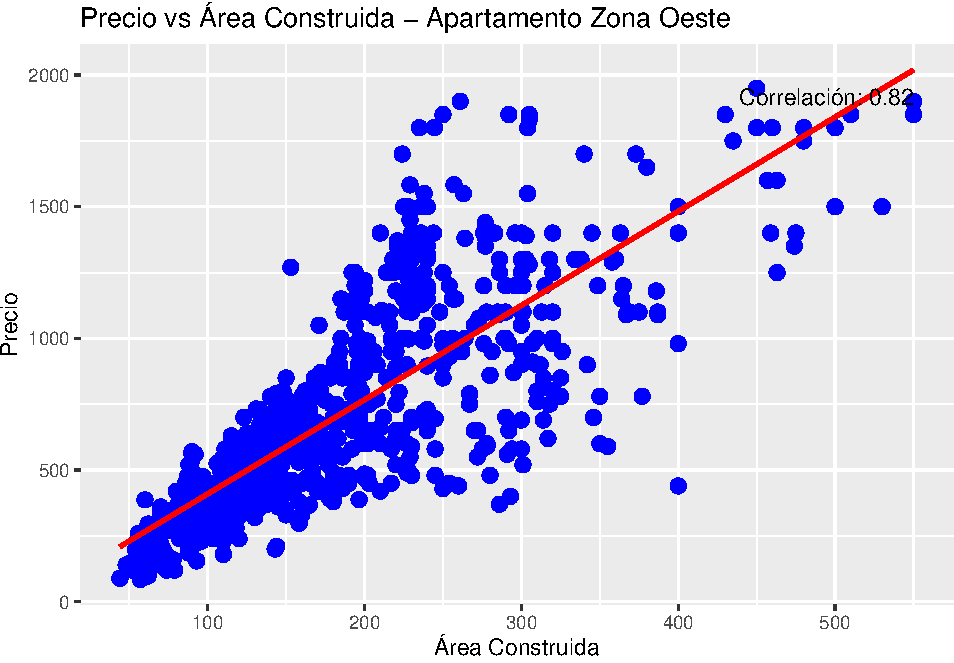
\includegraphics{A2_U2_InformeEjecutivo_files/figure-latex/unnamed-chunk-26-1.pdf}
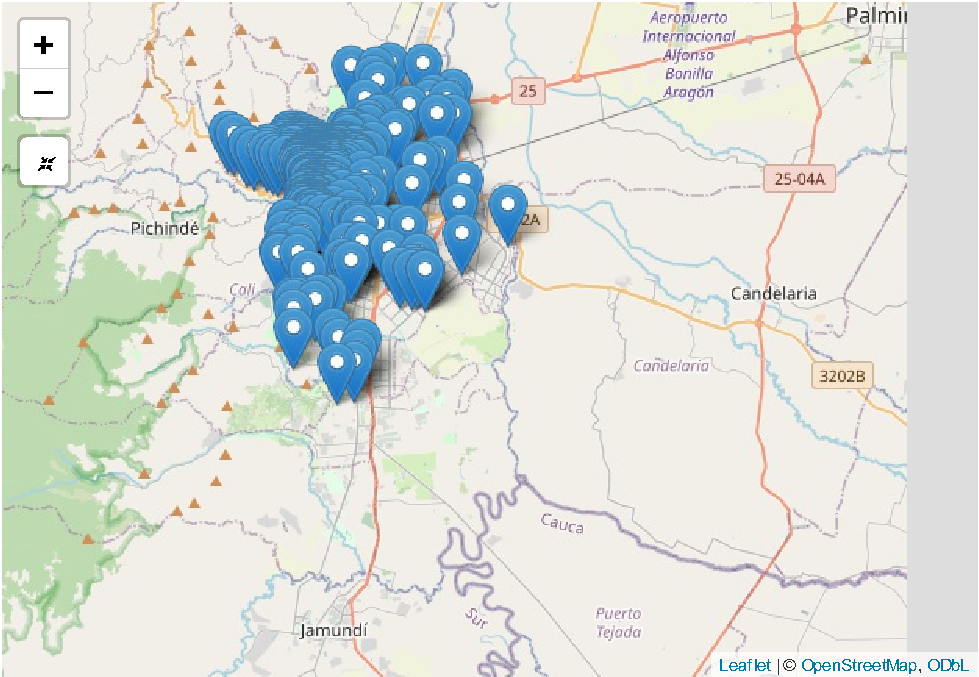
\includegraphics{A2_U2_InformeEjecutivo_files/figure-latex/unnamed-chunk-26-2.pdf}

Base 2 Apartamentos Zona Oeste

\begin{verbatim}
## Primeros 3 registros de la base de datos filtrada:
\end{verbatim}

\begin{longtable}[]{@{}
  >{\raggedleft\arraybackslash}p{(\columnwidth - 24\tabcolsep) * \real{0.0417}}
  >{\raggedright\arraybackslash}p{(\columnwidth - 24\tabcolsep) * \real{0.0917}}
  >{\raggedright\arraybackslash}p{(\columnwidth - 24\tabcolsep) * \real{0.0417}}
  >{\raggedleft\arraybackslash}p{(\columnwidth - 24\tabcolsep) * \real{0.0667}}
  >{\raggedleft\arraybackslash}p{(\columnwidth - 24\tabcolsep) * \real{0.0667}}
  >{\raggedleft\arraybackslash}p{(\columnwidth - 24\tabcolsep) * \real{0.0833}}
  >{\raggedleft\arraybackslash}p{(\columnwidth - 24\tabcolsep) * \real{0.1083}}
  >{\raggedleft\arraybackslash}p{(\columnwidth - 24\tabcolsep) * \real{0.0583}}
  >{\raggedleft\arraybackslash}p{(\columnwidth - 24\tabcolsep) * \real{0.1083}}
  >{\raggedright\arraybackslash}p{(\columnwidth - 24\tabcolsep) * \real{0.1000}}
  >{\raggedright\arraybackslash}p{(\columnwidth - 24\tabcolsep) * \real{0.0833}}
  >{\raggedleft\arraybackslash}p{(\columnwidth - 24\tabcolsep) * \real{0.0833}}
  >{\raggedleft\arraybackslash}p{(\columnwidth - 24\tabcolsep) * \real{0.0667}}@{}}
\toprule\noalign{}
\begin{minipage}[b]{\linewidth}\raggedleft
id
\end{minipage} & \begin{minipage}[b]{\linewidth}\raggedright
zona
\end{minipage} & \begin{minipage}[b]{\linewidth}\raggedright
piso
\end{minipage} & \begin{minipage}[b]{\linewidth}\raggedleft
estrato
\end{minipage} & \begin{minipage}[b]{\linewidth}\raggedleft
preciom
\end{minipage} & \begin{minipage}[b]{\linewidth}\raggedleft
areaconst
\end{minipage} & \begin{minipage}[b]{\linewidth}\raggedleft
parqueaderos
\end{minipage} & \begin{minipage}[b]{\linewidth}\raggedleft
banios
\end{minipage} & \begin{minipage}[b]{\linewidth}\raggedleft
habitaciones
\end{minipage} & \begin{minipage}[b]{\linewidth}\raggedright
tipo
\end{minipage} & \begin{minipage}[b]{\linewidth}\raggedright
barrio
\end{minipage} & \begin{minipage}[b]{\linewidth}\raggedleft
longitud
\end{minipage} & \begin{minipage}[b]{\linewidth}\raggedleft
latitud
\end{minipage} \\
\midrule\noalign{}
\endhead
\bottomrule\noalign{}
\endlastfoot
6999 & Zona Oeste & 01 & 6 & 870 & 200 & 2 & 5 & 3 & Apartamento &
aguacatal & -76.54666 & 3.44624 \\
8037 & Zona Oeste & 01 & 4 & 130 & 50 & NA & 1 & 3 & Apartamento &
aguacatal & -76.55409 & 3.44338 \\
8055 & Zona Oeste & 01 & 4 & 165 & 61 & 1 & 2 & 3 & Apartamento &
aguacatal & -76.55447 & 3.45783 \\
\end{longtable}

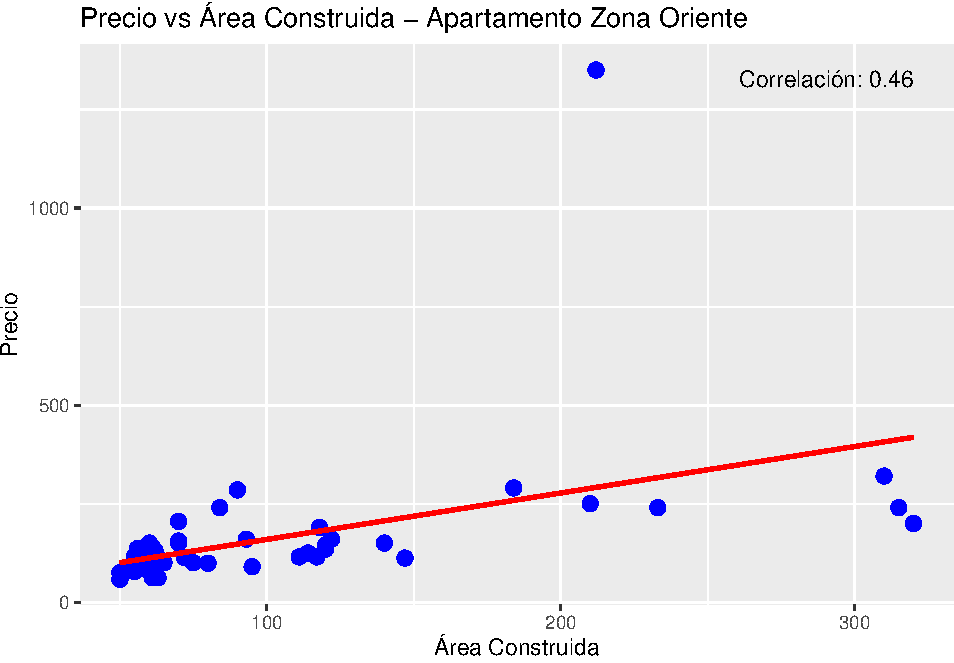
\includegraphics{A2_U2_InformeEjecutivo_files/figure-latex/unnamed-chunk-27-1.pdf}
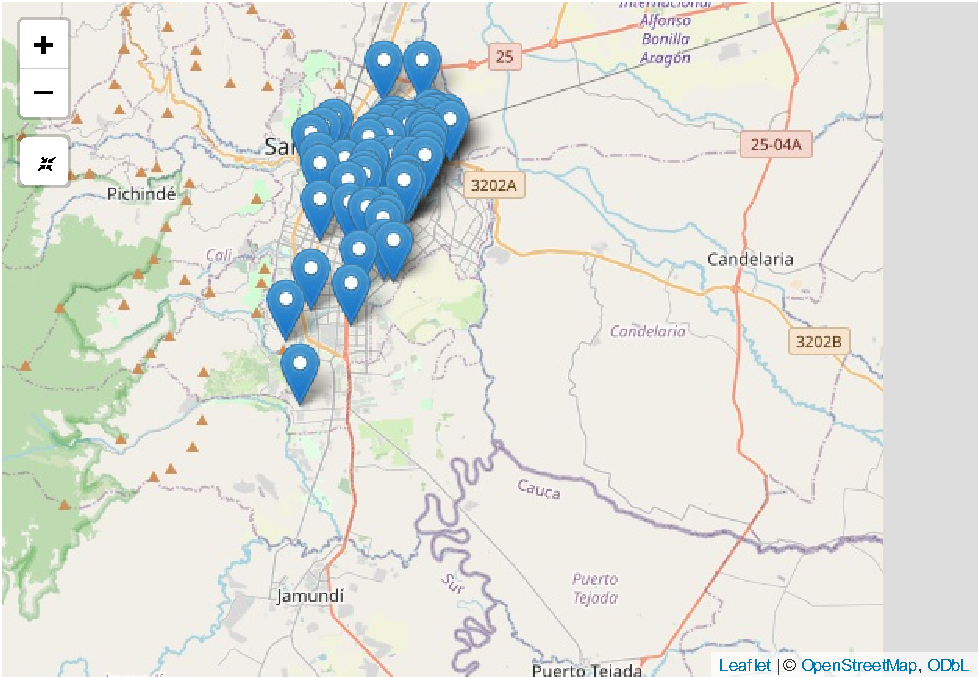
\includegraphics{A2_U2_InformeEjecutivo_files/figure-latex/unnamed-chunk-27-2.pdf}

Base 2 Apartamentos Zona Oriente

\begin{verbatim}
## Primeros 3 registros de la base de datos filtrada:
\end{verbatim}

\begin{longtable}[]{@{}
  >{\raggedleft\arraybackslash}p{(\columnwidth - 24\tabcolsep) * \real{0.0310}}
  >{\raggedright\arraybackslash}p{(\columnwidth - 24\tabcolsep) * \real{0.1008}}
  >{\raggedright\arraybackslash}p{(\columnwidth - 24\tabcolsep) * \real{0.0388}}
  >{\raggedleft\arraybackslash}p{(\columnwidth - 24\tabcolsep) * \real{0.0620}}
  >{\raggedleft\arraybackslash}p{(\columnwidth - 24\tabcolsep) * \real{0.0620}}
  >{\raggedleft\arraybackslash}p{(\columnwidth - 24\tabcolsep) * \real{0.0775}}
  >{\raggedleft\arraybackslash}p{(\columnwidth - 24\tabcolsep) * \real{0.1008}}
  >{\raggedleft\arraybackslash}p{(\columnwidth - 24\tabcolsep) * \real{0.0543}}
  >{\raggedleft\arraybackslash}p{(\columnwidth - 24\tabcolsep) * \real{0.1008}}
  >{\raggedright\arraybackslash}p{(\columnwidth - 24\tabcolsep) * \real{0.0930}}
  >{\raggedright\arraybackslash}p{(\columnwidth - 24\tabcolsep) * \real{0.1395}}
  >{\raggedleft\arraybackslash}p{(\columnwidth - 24\tabcolsep) * \real{0.0775}}
  >{\raggedleft\arraybackslash}p{(\columnwidth - 24\tabcolsep) * \real{0.0620}}@{}}
\toprule\noalign{}
\begin{minipage}[b]{\linewidth}\raggedleft
id
\end{minipage} & \begin{minipage}[b]{\linewidth}\raggedright
zona
\end{minipage} & \begin{minipage}[b]{\linewidth}\raggedright
piso
\end{minipage} & \begin{minipage}[b]{\linewidth}\raggedleft
estrato
\end{minipage} & \begin{minipage}[b]{\linewidth}\raggedleft
preciom
\end{minipage} & \begin{minipage}[b]{\linewidth}\raggedleft
areaconst
\end{minipage} & \begin{minipage}[b]{\linewidth}\raggedleft
parqueaderos
\end{minipage} & \begin{minipage}[b]{\linewidth}\raggedleft
banios
\end{minipage} & \begin{minipage}[b]{\linewidth}\raggedleft
habitaciones
\end{minipage} & \begin{minipage}[b]{\linewidth}\raggedright
tipo
\end{minipage} & \begin{minipage}[b]{\linewidth}\raggedright
barrio
\end{minipage} & \begin{minipage}[b]{\linewidth}\raggedleft
longitud
\end{minipage} & \begin{minipage}[b]{\linewidth}\raggedleft
latitud
\end{minipage} \\
\midrule\noalign{}
\endhead
\bottomrule\noalign{}
\endlastfoot
82 & Zona Oriente & 01 & 3 & 115 & 111 & 1 & 2 & 4 & Apartamento &
alfonso lópez & -76.48141 & 3.45379 \\
78 & Zona Oriente & 02 & 3 & 58 & 50 & 1 & 1 & 2 & Apartamento & alfonso
lópez & -76.47978 & 3.45131 \\
999 & Zona Oriente & 02 & 3 & 135 & 120 & NA & 2 & 4 & Apartamento &
atanasio girardot & -76.50737 & 3.44454 \\
\end{longtable}

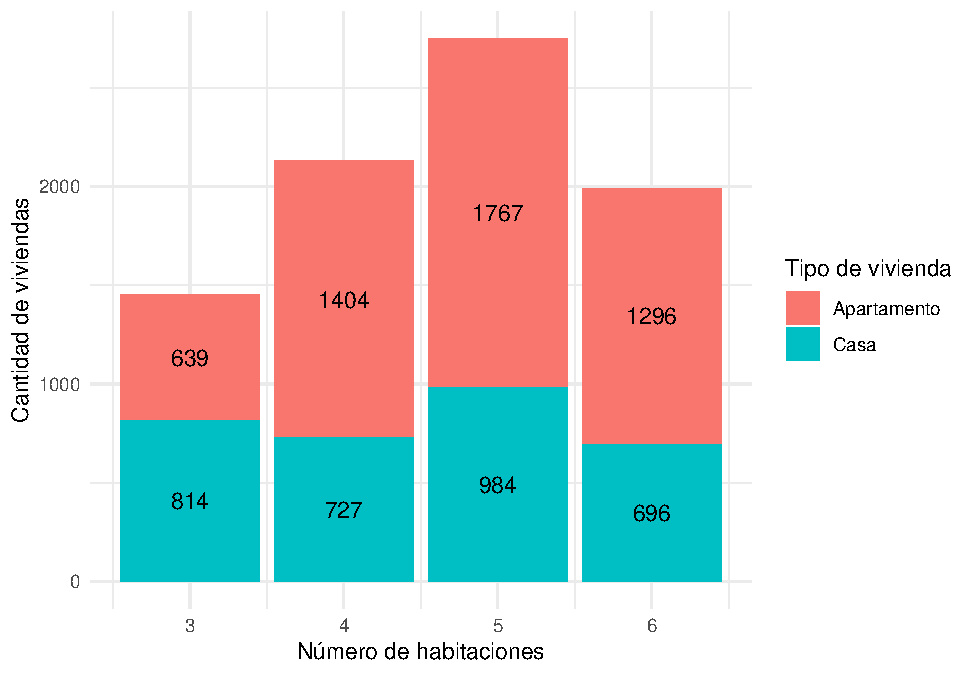
\includegraphics{A2_U2_InformeEjecutivo_files/figure-latex/unnamed-chunk-28-1.pdf}
\includegraphics{A2_U2_InformeEjecutivo_files/figure-latex/unnamed-chunk-28-2.pdf}

Base 2 Apartamentos Zona Centro

\begin{verbatim}
## Primeros 3 registros de la base de datos filtrada:
\end{verbatim}

\begin{longtable}[]{@{}
  >{\raggedleft\arraybackslash}p{(\columnwidth - 24\tabcolsep) * \real{0.0420}}
  >{\raggedright\arraybackslash}p{(\columnwidth - 24\tabcolsep) * \real{0.1008}}
  >{\raggedright\arraybackslash}p{(\columnwidth - 24\tabcolsep) * \real{0.0420}}
  >{\raggedleft\arraybackslash}p{(\columnwidth - 24\tabcolsep) * \real{0.0672}}
  >{\raggedleft\arraybackslash}p{(\columnwidth - 24\tabcolsep) * \real{0.0672}}
  >{\raggedleft\arraybackslash}p{(\columnwidth - 24\tabcolsep) * \real{0.0840}}
  >{\raggedleft\arraybackslash}p{(\columnwidth - 24\tabcolsep) * \real{0.1092}}
  >{\raggedleft\arraybackslash}p{(\columnwidth - 24\tabcolsep) * \real{0.0588}}
  >{\raggedleft\arraybackslash}p{(\columnwidth - 24\tabcolsep) * \real{0.1092}}
  >{\raggedright\arraybackslash}p{(\columnwidth - 24\tabcolsep) * \real{0.1008}}
  >{\raggedright\arraybackslash}p{(\columnwidth - 24\tabcolsep) * \real{0.0672}}
  >{\raggedleft\arraybackslash}p{(\columnwidth - 24\tabcolsep) * \real{0.0840}}
  >{\raggedleft\arraybackslash}p{(\columnwidth - 24\tabcolsep) * \real{0.0672}}@{}}
\toprule\noalign{}
\begin{minipage}[b]{\linewidth}\raggedleft
id
\end{minipage} & \begin{minipage}[b]{\linewidth}\raggedright
zona
\end{minipage} & \begin{minipage}[b]{\linewidth}\raggedright
piso
\end{minipage} & \begin{minipage}[b]{\linewidth}\raggedleft
estrato
\end{minipage} & \begin{minipage}[b]{\linewidth}\raggedleft
preciom
\end{minipage} & \begin{minipage}[b]{\linewidth}\raggedleft
areaconst
\end{minipage} & \begin{minipage}[b]{\linewidth}\raggedleft
parqueaderos
\end{minipage} & \begin{minipage}[b]{\linewidth}\raggedleft
banios
\end{minipage} & \begin{minipage}[b]{\linewidth}\raggedleft
habitaciones
\end{minipage} & \begin{minipage}[b]{\linewidth}\raggedright
tipo
\end{minipage} & \begin{minipage}[b]{\linewidth}\raggedright
barrio
\end{minipage} & \begin{minipage}[b]{\linewidth}\raggedleft
longitud
\end{minipage} & \begin{minipage}[b]{\linewidth}\raggedleft
latitud
\end{minipage} \\
\midrule\noalign{}
\endhead
\bottomrule\noalign{}
\endlastfoot
4654 & Zona Centro & 03 & 3 & 100 & 70.00 & NA & 2 & 3 & Apartamento &
alameda & -76.53200 & 3.45200 \\
4408 & Zona Centro & 05 & 3 & 120 & 84.00 & 1 & 2 & 3 & Apartamento &
alameda & -76.53123 & 3.44011 \\
4395 & Zona Centro & 04 & 3 & 125 & 66.76 & NA & 2 & 3 & Apartamento &
bretaña & -76.53111 & 3.44034 \\
\end{longtable}

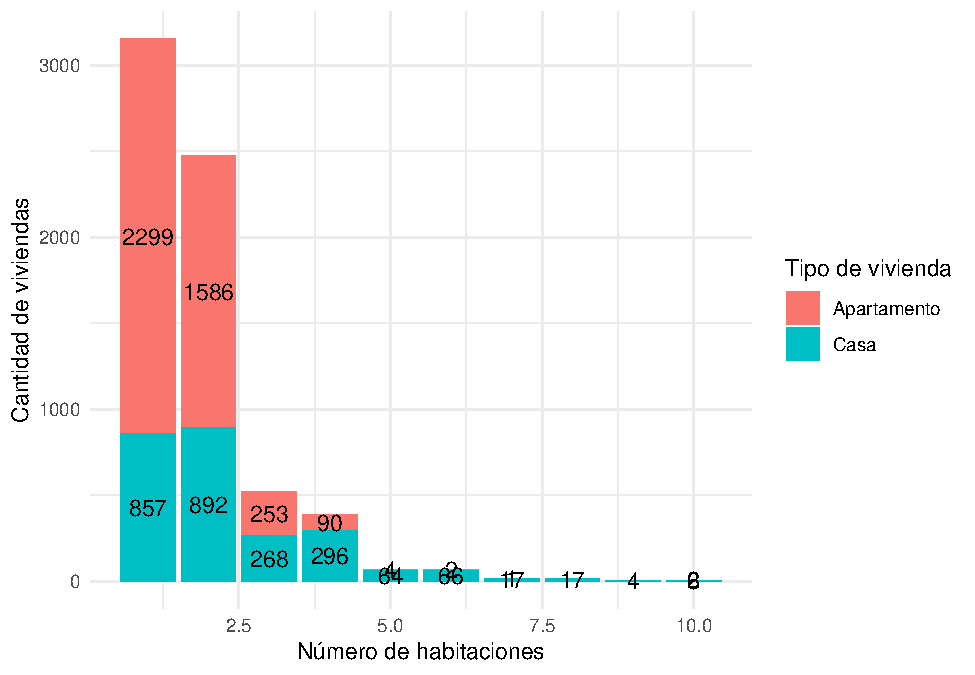
\includegraphics{A2_U2_InformeEjecutivo_files/figure-latex/unnamed-chunk-29-1.pdf}
\includegraphics{A2_U2_InformeEjecutivo_files/figure-latex/unnamed-chunk-29-2.pdf}

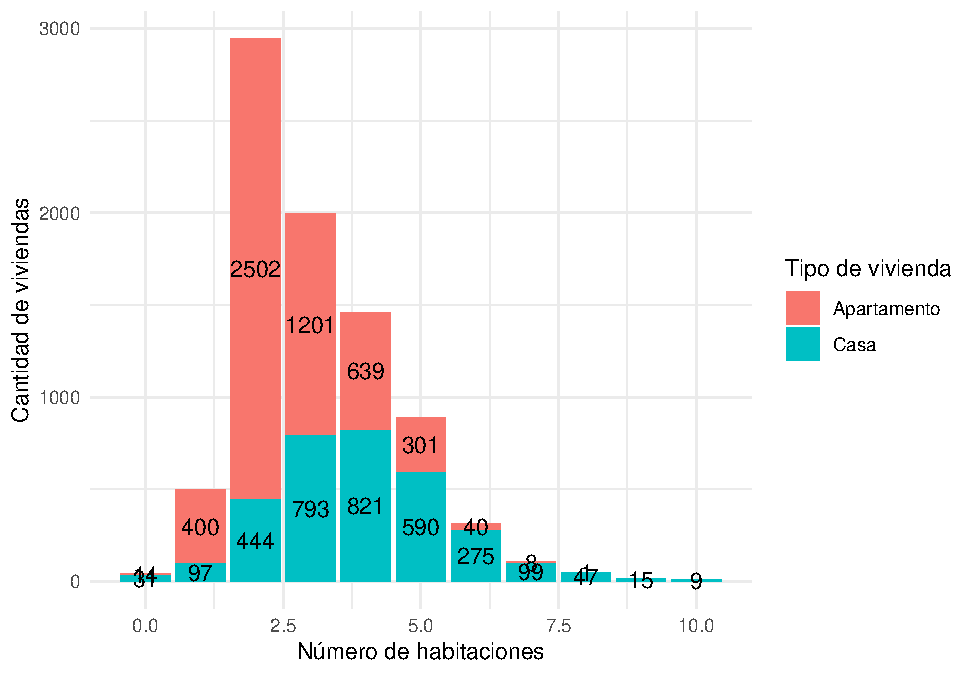
\includegraphics{A2_U2_InformeEjecutivo_files/figure-latex/unnamed-chunk-30-1.pdf}

Basado en la información generada se identifica que según el gráfico de
dispersión: La zona oeste presenta la mayor concentración de puntos en
la zona superior derecha, lo que indica una mayor cantidad de
propiedades con precios elevados y áreas construidas amplias. de otra
parte el rango de precios para la zona oeste es el más alto, por tanto,
la zona oeste tiene el coeficiente de correlación más fuerte (0.82), lo
que indica una relación más estrecha entre precio y área construida.

Ahora hablando de la comparación con otras zonas, se observa que la Zona
Sur aunque tiene un coeficiente de correlación similar a la zona norte
(0.76), el rango de precios es ligeramente inferior. La Zona Norte: Si
bien presenta un rango de precios similar a la zona sur, la
concentración de puntos en la zona superior derecha del gráfico de
dispersión es menor. Por su parte la Zona Oriente es la que presenta los
precios más bajos, aunque presenta un dato atípico en la gráfica este no
altera la tendencia general de precios más bajos. Por ultimo la Zona
Centro Ofrece precios intermedios, con una poca oferta inmoboliaria
respecto a Apartamento, esto puede deberse a la dinamica comercial
propia del sector reduciendo la vivienda residencial.

Tambien es valido destacar que al igual con los datos registrados en el
tipo de vivienda ``Casa'' se evidencia un error humano en la asignación
del tipo de zona o en los datos de longitud y latitud dado que en el
ultimo grafico se observa que existen traslapos en los colores, esto
sucede con mayor incidencia en la parte superior del mapa.

Analisis exploratorio

\begin{verbatim}
##        id           zona               piso              estrato     
##  Min.   :   3   Length:5100        Length:5100        Min.   :3.000  
##  1st Qu.:2180   Class :character   Class :character   1st Qu.:4.000  
##  Median :4158   Mode  :character   Mode  :character   Median :5.000  
##  Mean   :4284                                         Mean   :4.727  
##  3rd Qu.:6556                                         3rd Qu.:6.000  
##  Max.   :8317                                         Max.   :6.000  
##                                                                      
##     preciom         areaconst      parqueaderos        banios     
##  Min.   :  58.0   Min.   : 35.0   Min.   : 1.000   Min.   :0.000  
##  1st Qu.: 175.0   1st Qu.: 68.0   1st Qu.: 1.000   1st Qu.:2.000  
##  Median : 279.0   Median : 90.0   Median : 1.000   Median :2.000  
##  Mean   : 366.9   Mean   :112.8   Mean   : 1.568   Mean   :2.617  
##  3rd Qu.: 430.0   3rd Qu.:130.0   3rd Qu.: 2.000   3rd Qu.:3.000  
##  Max.   :1950.0   Max.   :932.0   Max.   :10.000   Max.   :8.000  
##                                   NA's   :869                     
##   habitaciones       tipo              barrio             longitud     
##  Min.   :0.000   Length:5100        Length:5100        Min.   :-76.59  
##  1st Qu.:3.000   Class :character   Class :character   1st Qu.:-76.54  
##  Median :3.000   Mode  :character   Mode  :character   Median :-76.53  
##  Mean   :2.971                                         Mean   :-76.53  
##  3rd Qu.:3.000                                         3rd Qu.:-76.52  
##  Max.   :9.000                                         Max.   :-76.46  
##                                                                        
##     latitud     
##  Min.   :3.334  
##  1st Qu.:3.380  
##  Median :3.419  
##  Mean   :3.419  
##  3rd Qu.:3.453  
##  Max.   :3.498  
## 
\end{verbatim}

\begin{verbatim}
## tibble [5,100 x 13] (S3: tbl_df/tbl/data.frame)
##  $ id          : num [1:5100] 1212 1724 2326 4386 7497 ...
##  $ zona        : chr [1:5100] "Zona Norte" "Zona Norte" "Zona Norte" "Zona Norte" ...
##  $ piso        : chr [1:5100] "01" "01" "01" "01" ...
##  $ estrato     : num [1:5100] 5 5 4 5 6 4 5 3 3 6 ...
##  $ preciom     : num [1:5100] 260 240 220 310 520 320 385 100 175 820 ...
##  $ areaconst   : num [1:5100] 90 87 52 137 98 108 103 49 80 377 ...
##  $ parqueaderos: num [1:5100] 1 1 2 2 2 2 2 NA 1 1 ...
##  $ banios      : num [1:5100] 2 3 2 3 2 3 2 1 2 4 ...
##  $ habitaciones: num [1:5100] 3 3 3 4 2 3 3 2 3 4 ...
##  $ tipo        : chr [1:5100] "Apartamento" "Apartamento" "Apartamento" "Apartamento" ...
##  $ barrio      : chr [1:5100] "acopi" "acopi" "acopi" "acopi" ...
##  $ longitud    : num [1:5100] -76.5 -76.5 -76.5 -76.5 -76.5 ...
##  $ latitud     : num [1:5100] 3.46 3.37 3.43 3.38 3.44 ...
\end{verbatim}

\begin{verbatim}
##        id          estrato         preciom         areaconst    
##  Min.   :   3   Min.   :3.000   Min.   :  58.0   Min.   : 35.0  
##  1st Qu.:2180   1st Qu.:4.000   1st Qu.: 175.0   1st Qu.: 68.0  
##  Median :4158   Median :5.000   Median : 279.0   Median : 90.0  
##  Mean   :4284   Mean   :4.727   Mean   : 366.9   Mean   :112.8  
##  3rd Qu.:6556   3rd Qu.:6.000   3rd Qu.: 430.0   3rd Qu.:130.0  
##  Max.   :8317   Max.   :6.000   Max.   :1950.0   Max.   :932.0  
##                                                                 
##   parqueaderos        banios       habitaciones      longitud     
##  Min.   : 1.000   Min.   :0.000   Min.   :0.000   Min.   :-76.59  
##  1st Qu.: 1.000   1st Qu.:2.000   1st Qu.:3.000   1st Qu.:-76.54  
##  Median : 1.000   Median :2.000   Median :3.000   Median :-76.53  
##  Mean   : 1.568   Mean   :2.617   Mean   :2.971   Mean   :-76.53  
##  3rd Qu.: 2.000   3rd Qu.:3.000   3rd Qu.:3.000   3rd Qu.:-76.52  
##  Max.   :10.000   Max.   :8.000   Max.   :9.000   Max.   :-76.46  
##  NA's   :869                                                      
##     latitud     
##  Min.   :3.334  
##  1st Qu.:3.380  
##  Median :3.419  
##  Mean   :3.419  
##  3rd Qu.:3.453  
##  Max.   :3.498  
## 
\end{verbatim}

\begin{verbatim}
## < table of extent 0 x 0 >
\end{verbatim}

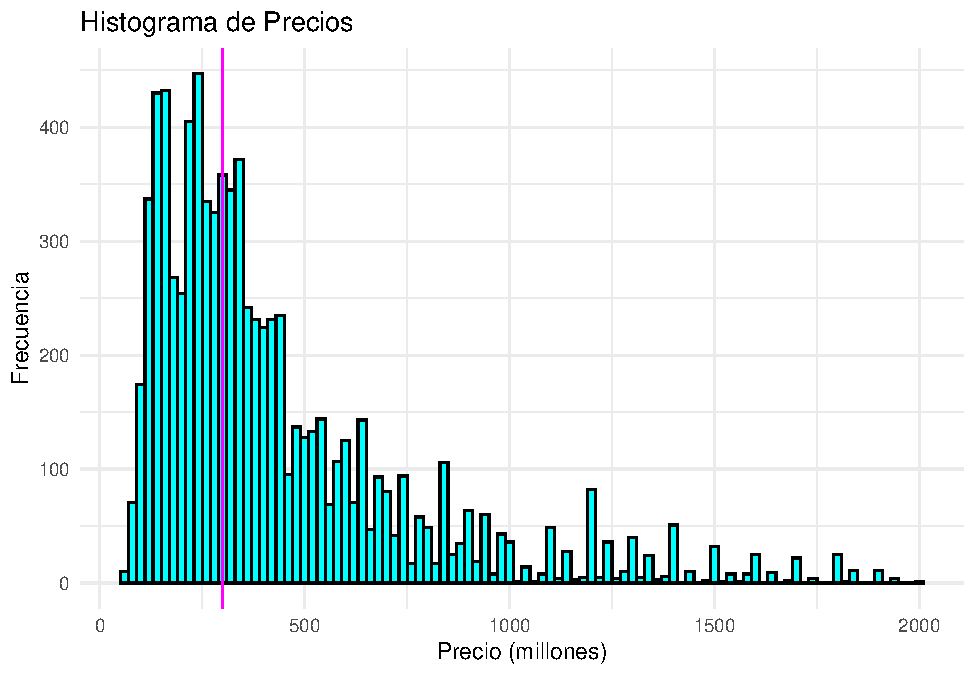
\includegraphics{A2_U2_InformeEjecutivo_files/figure-latex/unnamed-chunk-32-1.pdf}
\includegraphics{A2_U2_InformeEjecutivo_files/figure-latex/unnamed-chunk-32-2.pdf}

\begin{verbatim}
## $preciom
##               Df    Sum Sq  Mean Sq F value Pr(>F)    
## zona           4 118380819 29595205   489.3 <2e-16 ***
## Residuals   5095 308139573    60479                   
## ---
## Signif. codes:  0 '***' 0.001 '**' 0.01 '*' 0.05 '.' 0.1 ' ' 1
## 
## $areaconst
##               Df   Sum Sq Mean Sq F value Pr(>F)    
## zona           4  4566161 1141540   291.3 <2e-16 ***
## Residuals   5095 19963328    3918                   
## ---
## Signif. codes:  0 '***' 0.001 '**' 0.01 '*' 0.05 '.' 0.1 ' ' 1
## 
## $estrato
##               Df Sum Sq Mean Sq F value Pr(>F)    
## zona           4   1156  289.03   396.3 <2e-16 ***
## Residuals   5095   3715    0.73                   
## ---
## Signif. codes:  0 '***' 0.001 '**' 0.01 '*' 0.05 '.' 0.1 ' ' 1
## 
## $banios
##               Df Sum Sq Mean Sq F value Pr(>F)    
## zona           4    827  206.79   210.9 <2e-16 ***
## Residuals   5095   4996    0.98                   
## ---
## Signif. codes:  0 '***' 0.001 '**' 0.01 '*' 0.05 '.' 0.1 ' ' 1
## 
## $habitaciones
##               Df Sum Sq Mean Sq F value   Pr(>F)    
## zona           4     18   4.508   9.935 5.25e-08 ***
## Residuals   5095   2312   0.454                     
## ---
## Signif. codes:  0 '***' 0.001 '**' 0.01 '*' 0.05 '.' 0.1 ' ' 1
\end{verbatim}

\begin{longtable}[]{@{}ll@{}}
\caption{Data summary}\tabularnewline
\toprule\noalign{}
\endfirsthead
\endhead
\bottomrule\noalign{}
\endlastfoot
Name & vivienda\_apartamento \\
Number of rows & 5100 \\
Number of columns & 13 \\
\_\_\_\_\_\_\_\_\_\_\_\_\_\_\_\_\_\_\_\_\_\_\_ & \\
Column type frequency: & \\
character & 4 \\
numeric & 9 \\
\_\_\_\_\_\_\_\_\_\_\_\_\_\_\_\_\_\_\_\_\_\_\_\_ & \\
Group variables & None \\
\end{longtable}

\textbf{Variable type: character}

\begin{longtable}[]{@{}
  >{\raggedright\arraybackslash}p{(\columnwidth - 14\tabcolsep) * \real{0.1944}}
  >{\raggedleft\arraybackslash}p{(\columnwidth - 14\tabcolsep) * \real{0.1389}}
  >{\raggedleft\arraybackslash}p{(\columnwidth - 14\tabcolsep) * \real{0.1944}}
  >{\raggedleft\arraybackslash}p{(\columnwidth - 14\tabcolsep) * \real{0.0556}}
  >{\raggedleft\arraybackslash}p{(\columnwidth - 14\tabcolsep) * \real{0.0556}}
  >{\raggedleft\arraybackslash}p{(\columnwidth - 14\tabcolsep) * \real{0.0833}}
  >{\raggedleft\arraybackslash}p{(\columnwidth - 14\tabcolsep) * \real{0.1250}}
  >{\raggedleft\arraybackslash}p{(\columnwidth - 14\tabcolsep) * \real{0.1528}}@{}}
\toprule\noalign{}
\begin{minipage}[b]{\linewidth}\raggedright
skim\_variable
\end{minipage} & \begin{minipage}[b]{\linewidth}\raggedleft
n\_missing
\end{minipage} & \begin{minipage}[b]{\linewidth}\raggedleft
complete\_rate
\end{minipage} & \begin{minipage}[b]{\linewidth}\raggedleft
min
\end{minipage} & \begin{minipage}[b]{\linewidth}\raggedleft
max
\end{minipage} & \begin{minipage}[b]{\linewidth}\raggedleft
empty
\end{minipage} & \begin{minipage}[b]{\linewidth}\raggedleft
n\_unique
\end{minipage} & \begin{minipage}[b]{\linewidth}\raggedleft
whitespace
\end{minipage} \\
\midrule\noalign{}
\endhead
\bottomrule\noalign{}
\endlastfoot
zona & 0 & 1.00 & 8 & 12 & 0 & 5 & 0 \\
piso & 1381 & 0.73 & 2 & 2 & 0 & 12 & 0 \\
tipo & 0 & 1.00 & 11 & 11 & 0 & 1 & 0 \\
barrio & 0 & 1.00 & 4 & 29 & 0 & 289 & 0 \\
\end{longtable}

\textbf{Variable type: numeric}

\begin{longtable}[]{@{}
  >{\raggedright\arraybackslash}p{(\columnwidth - 20\tabcolsep) * \real{0.1414}}
  >{\raggedleft\arraybackslash}p{(\columnwidth - 20\tabcolsep) * \real{0.1010}}
  >{\raggedleft\arraybackslash}p{(\columnwidth - 20\tabcolsep) * \real{0.1414}}
  >{\raggedleft\arraybackslash}p{(\columnwidth - 20\tabcolsep) * \real{0.0808}}
  >{\raggedleft\arraybackslash}p{(\columnwidth - 20\tabcolsep) * \real{0.0808}}
  >{\raggedleft\arraybackslash}p{(\columnwidth - 20\tabcolsep) * \real{0.0707}}
  >{\raggedleft\arraybackslash}p{(\columnwidth - 20\tabcolsep) * \real{0.0808}}
  >{\raggedleft\arraybackslash}p{(\columnwidth - 20\tabcolsep) * \real{0.0808}}
  >{\raggedleft\arraybackslash}p{(\columnwidth - 20\tabcolsep) * \real{0.0808}}
  >{\raggedleft\arraybackslash}p{(\columnwidth - 20\tabcolsep) * \real{0.0808}}
  >{\raggedright\arraybackslash}p{(\columnwidth - 20\tabcolsep) * \real{0.0606}}@{}}
\toprule\noalign{}
\begin{minipage}[b]{\linewidth}\raggedright
skim\_variable
\end{minipage} & \begin{minipage}[b]{\linewidth}\raggedleft
n\_missing
\end{minipage} & \begin{minipage}[b]{\linewidth}\raggedleft
complete\_rate
\end{minipage} & \begin{minipage}[b]{\linewidth}\raggedleft
mean
\end{minipage} & \begin{minipage}[b]{\linewidth}\raggedleft
sd
\end{minipage} & \begin{minipage}[b]{\linewidth}\raggedleft
p0
\end{minipage} & \begin{minipage}[b]{\linewidth}\raggedleft
p25
\end{minipage} & \begin{minipage}[b]{\linewidth}\raggedleft
p50
\end{minipage} & \begin{minipage}[b]{\linewidth}\raggedleft
p75
\end{minipage} & \begin{minipage}[b]{\linewidth}\raggedleft
p100
\end{minipage} & \begin{minipage}[b]{\linewidth}\raggedright
hist
\end{minipage} \\
\midrule\noalign{}
\endhead
\bottomrule\noalign{}
\endlastfoot
id & 0 & 1.00 & 4284.03 & 2449.82 & 3.00 & 2179.75 & 4158.50 & 6556.25 &
8317.00 & ▆▇▆▆▇ \\
estrato & 0 & 1.00 & 4.73 & 0.98 & 3.00 & 4.00 & 5.00 & 6.00 & 6.00 &
▃▆▁▇▆ \\
preciom & 0 & 1.00 & 366.94 & 289.22 & 58.00 & 175.00 & 279.00 & 430.00
& 1950.00 & ▇▂▁▁▁ \\
areaconst & 0 & 1.00 & 112.78 & 69.36 & 35.00 & 68.00 & 90.00 & 130.00 &
932.00 & ▇▁▁▁▁ \\
parqueaderos & 869 & 0.83 & 1.57 & 0.74 & 1.00 & 1.00 & 1.00 & 2.00 &
10.00 & ▇▁▁▁▁ \\
banios & 0 & 1.00 & 2.62 & 1.07 & 0.00 & 2.00 & 2.00 & 3.00 & 8.00 &
▁▇▂▁▁ \\
habitaciones & 0 & 1.00 & 2.97 & 0.68 & 0.00 & 3.00 & 3.00 & 3.00 & 9.00
& ▁▇▂▁▁ \\
longitud & 0 & 1.00 & -76.53 & 0.02 & -76.59 & -76.54 & -76.53 & -76.52
& -76.46 & ▁▅▇▂▁ \\
latitud & 0 & 1.00 & 3.42 & 0.04 & 3.33 & 3.38 & 3.42 & 3.45 & 3.50 &
▂▇▅▇▅ \\
\end{longtable}

Interpretación del Modelo El modelo de regresión lineal múltiple
ajustado es:

Precio = β0 + β1 * Área Construida + β2 * Estrato + β3 * Parqueaderos +
β4 * Baños + β5 * Habitaciones + ε

Donde:

β0 es el intercepto, que representa el precio esperado cuando todas las
demás variables son cero. β1, β2, β3, β4 y β5 son los coeficientes de
regresión que representan el cambio esperado en el precio para un
aumento unitario en cada variable, manteniendo todas las demás variables
constantes. ε es el término de error.

\begin{verbatim}
## 
## Call:
## lm(formula = preciom ~ areaconst + estrato + banios + habitaciones + 
##     zona, data = vivienda_apartamento_seleccion)
## 
## Residuals:
##      Min       1Q   Median       3Q      Max 
## -1904.61   -51.00     1.05    45.20   971.19 
## 
## Coefficients:
##                    Estimate Std. Error t value Pr(>|t|)    
## (Intercept)      -257.42194   29.85912  -8.621  < 2e-16 ***
## areaconst           2.22296    0.04204  52.873  < 2e-16 ***
## estrato            56.91854    2.68697  21.183  < 2e-16 ***
## banios             61.11292    2.99576  20.400  < 2e-16 ***
## habitaciones      -32.93022    3.32925  -9.891  < 2e-16 ***
## zonaZona Norte     31.08865   27.80772   1.118    0.264    
## zonaZona Oeste    118.86179   28.15735   4.221 2.47e-05 ***
## zonaZona Oriente   19.31989   32.37714   0.597    0.551    
## zonaZona Sur       20.09085   27.71277   0.725    0.469    
## ---
## Signif. codes:  0 '***' 0.001 '**' 0.01 '*' 0.05 '.' 0.1 ' ' 1
## 
## Residual standard error: 134.6 on 5091 degrees of freedom
## Multiple R-squared:  0.7839, Adjusted R-squared:  0.7836 
## F-statistic:  2308 on 8 and 5091 DF,  p-value: < 2.2e-16
\end{verbatim}

\begin{verbatim}
## El coeficiente para el área construida es: 2.222963
\end{verbatim}

\begin{verbatim}
## Los coeficientes para los estratos son: 56.91854
\end{verbatim}

\begin{verbatim}
## El coeficiente para los baños es: 61.11292
\end{verbatim}

\begin{verbatim}
## El coeficiente para las habitaciones es: -32.93022
\end{verbatim}

\begin{verbatim}
## Los coeficientes para las zonas son: 31.08865 118.8618 19.31989 20.09085
\end{verbatim}

\begin{verbatim}
## El R^2 del modelo es: 0.7838911
\end{verbatim}

El análisis del modelo de regresión aplicado revela que el precio de la
vivienda está influenciado significativamente por diversas
características. Por cada metro cuadrado adicional en el área
construida, el precio aumenta en aproximadamente \$2.22 millones.
Respecto a los estratos, se observa un aumento significativo en el
precio con valores cercanos a \$56.92 millones para estrato 6, mientras
que para los baños y habitaciones, se registra un incremento de
aproximadamente \$61.11 millones y una disminución de alrededor de
\$32.93 millones, respectivamente, por cada unidad adicional. En cuanto
a las zonas, se identifican variaciones de precios significativas,
siendo la Zona Sur la de mayor impacto con un incremento de \$118.86
millones, seguida por la Zona Norte con \$31.09 millones, la Zona Oeste
con \$20.09 millones y la Zona Centro con \$19.32 millones. El modelo
tiene un coeficiente de determinación (R\^{}2) de aproximadamente 0.78,
lo que indica que alrededor del 78.39\% de la variabilidad en el precio
de la vivienda puede ser explicada por las variables incluidas en el
modelo, demostrando un buen ajuste.

Validacion de supuestos

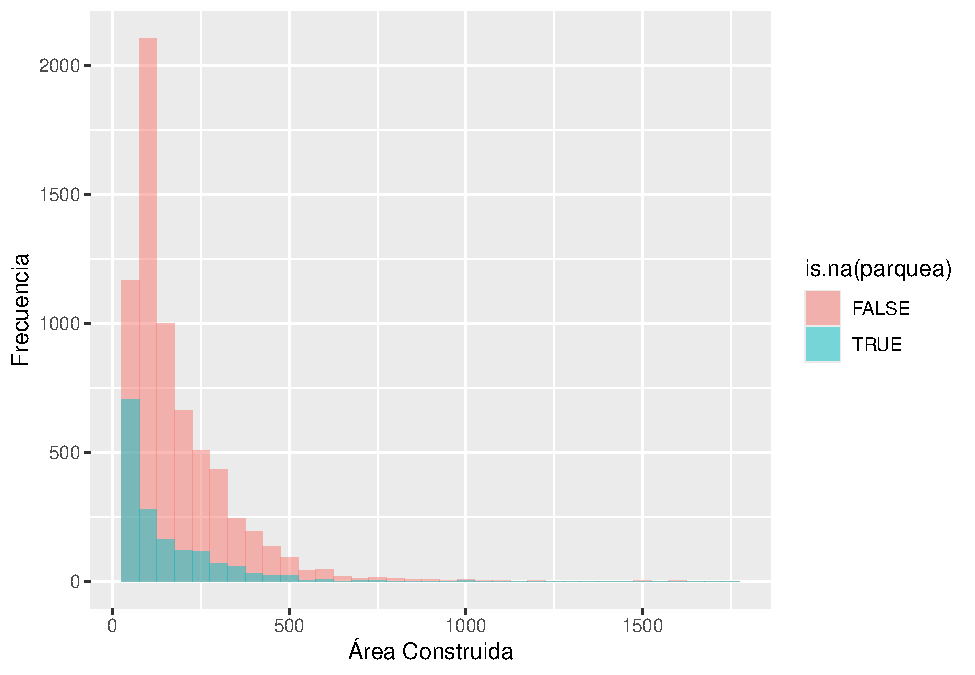
\includegraphics{A2_U2_InformeEjecutivo_files/figure-latex/unnamed-chunk-34-1.pdf}
\includegraphics{A2_U2_InformeEjecutivo_files/figure-latex/unnamed-chunk-34-2.pdf}

\begin{verbatim}
## 
##  studentized Breusch-Pagan test
## 
## data:  modelo_regresion
## BP = 1465.5, df = 8, p-value < 2.2e-16
\end{verbatim}

\begin{verbatim}
## 
##  Box-Ljung test
## 
## data:  modelo_regresion$resid
## X-squared = 127.18, df = 1, p-value < 2.2e-16
\end{verbatim}

Test de Breusch-Pagan para homocedasticidad: El valor de estadístico de
prueba (BP) es 1465.5 con 8 grados de libertad, y el p-valor es menor
que 2.2e-16. Esto indica que hay evidencia significativa para rechazar
la hipótesis nula de homocedasticidad, lo que sugiere que los residuos
no tienen varianza constante.

Test de Ljung-Box para autocorrelación de los residuos: El valor de
estadístico de prueba (X-squared) es 127.18 con 1 grado de libertad, y
el p-valor es menor que 2.2e-16. Esto indica que hay evidencia
significativa para rechazar la hipótesis nula de independencia de los
residuos, lo que sugiere que los residuos están autocorrelacionados.

Estos resultados pueden indicar que el modelo de regresión lineal
múltiple puede no cumplir completamente con los supuestos de
homocedasticidad e independencia de los residuos.

Predicción del precio

\begin{verbatim}
##        1        2 
## 732.8381 789.7567
\end{verbatim}

La predicción del precio para la vivienda especificada es de \$732.8381
millones (para el estrato 5) y \$789.7567 millones (para el estrato 6).

Potenciales ofertas

\begin{verbatim}
##   areaconst banios habitaciones estrato     zona precio_estimado
## 1       280      3            4       5 Zona Sur        721.3091
## 2       300      3            4       5 Zona Sur        765.7684
## 3       280      4            4       5 Zona Sur        782.4220
## 4       300      4            4       5 Zona Sur        826.8813
## 5       280      3            5       5 Zona Sur        688.3789
\end{verbatim}

Las ofertas potenciales presentan una variedad de opciones en términos
de tamaño, distribución de espacios y precios estimados. La primera
oferta, con un área construida de 280 metros cuadrados, ofrece 3 baños y
4 habitaciones, con un precio estimado de alrededor de \$721.31
millones. La segunda opción, también con 300 metros cuadrados, cuenta
con características similares pero un precio ligeramente superior,
aproximadamente \$765.77 millones. La tercera y cuarta oferta, con áreas
construidas de 280 y 300 metros cuadrados respectivamente, presentan 4
baños y 4 habitaciones, con precios estimados de \$782.42 y \$826.88
millones respectivamente. Finalmente, la quinta oferta, con 280 metros
cuadrados, ofrece 3 baños y 5 habitaciones, con el precio estimado más
bajo de todas, alrededor de \$688.38 millones. Estas opciones brindan a
los potenciales compradores una gama de alternativas para seleccionar la
vivienda que mejor se ajuste a sus necesidades y presupuesto.

\subsection{8. Anexos - Repositorio Código
fuente}\label{anexos---repositorio-cuxf3digo-fuente}

Repositorio Github

\end{document}
